
% Default to the notebook output style

    


% Inherit from the specified cell style.




    
\documentclass[11pt]{article}

    
    
    \usepackage[T1]{fontenc}
    % Nicer default font (+ math font) than Computer Modern for most use cases
    \usepackage{mathpazo}

    % Basic figure setup, for now with no caption control since it's done
    % automatically by Pandoc (which extracts ![](path) syntax from Markdown).
    \usepackage{graphicx}
    % We will generate all images so they have a width \maxwidth. This means
    % that they will get their normal width if they fit onto the page, but
    % are scaled down if they would overflow the margins.
    \makeatletter
    \def\maxwidth{\ifdim\Gin@nat@width>\linewidth\linewidth
    \else\Gin@nat@width\fi}
    \makeatother
    \let\Oldincludegraphics\includegraphics
    % Set max figure width to be 80% of text width, for now hardcoded.
    \renewcommand{\includegraphics}[1]{\Oldincludegraphics[width=.8\maxwidth]{#1}}
    % Ensure that by default, figures have no caption (until we provide a
    % proper Figure object with a Caption API and a way to capture that
    % in the conversion process - todo).
    \usepackage{caption}
    \DeclareCaptionLabelFormat{nolabel}{}
    \captionsetup{labelformat=nolabel}

    \usepackage{adjustbox} % Used to constrain images to a maximum size 
    \usepackage{xcolor} % Allow colors to be defined
    \usepackage{enumerate} % Needed for markdown enumerations to work
    \usepackage{geometry} % Used to adjust the document margins
    \usepackage{amsmath} % Equations
    \usepackage{amssymb} % Equations
    \usepackage{textcomp} % defines textquotesingle
    % Hack from http://tex.stackexchange.com/a/47451/13684:
    \AtBeginDocument{%
        \def\PYZsq{\textquotesingle}% Upright quotes in Pygmentized code
    }
    \usepackage{upquote} % Upright quotes for verbatim code
    \usepackage{eurosym} % defines \euro
    \usepackage[mathletters]{ucs} % Extended unicode (utf-8) support
    \usepackage[utf8x]{inputenc} % Allow utf-8 characters in the tex document
    \usepackage{fancyvrb} % verbatim replacement that allows latex
    \usepackage{grffile} % extends the file name processing of package graphics 
                         % to support a larger range 
    % The hyperref package gives us a pdf with properly built
    % internal navigation ('pdf bookmarks' for the table of contents,
    % internal cross-reference links, web links for URLs, etc.)
    \usepackage{hyperref}
    \usepackage{longtable} % longtable support required by pandoc >1.10
    \usepackage{booktabs}  % table support for pandoc > 1.12.2
    \usepackage[inline]{enumitem} % IRkernel/repr support (it uses the enumerate* environment)
    \usepackage[normalem]{ulem} % ulem is needed to support strikethroughs (\sout)
                                % normalem makes italics be italics, not underlines
    

    
    
    % Colors for the hyperref package
    \definecolor{urlcolor}{rgb}{0,.145,.698}
    \definecolor{linkcolor}{rgb}{.71,0.21,0.01}
    \definecolor{citecolor}{rgb}{.12,.54,.11}

    % ANSI colors
    \definecolor{ansi-black}{HTML}{3E424D}
    \definecolor{ansi-black-intense}{HTML}{282C36}
    \definecolor{ansi-red}{HTML}{E75C58}
    \definecolor{ansi-red-intense}{HTML}{B22B31}
    \definecolor{ansi-green}{HTML}{00A250}
    \definecolor{ansi-green-intense}{HTML}{007427}
    \definecolor{ansi-yellow}{HTML}{DDB62B}
    \definecolor{ansi-yellow-intense}{HTML}{B27D12}
    \definecolor{ansi-blue}{HTML}{208FFB}
    \definecolor{ansi-blue-intense}{HTML}{0065CA}
    \definecolor{ansi-magenta}{HTML}{D160C4}
    \definecolor{ansi-magenta-intense}{HTML}{A03196}
    \definecolor{ansi-cyan}{HTML}{60C6C8}
    \definecolor{ansi-cyan-intense}{HTML}{258F8F}
    \definecolor{ansi-white}{HTML}{C5C1B4}
    \definecolor{ansi-white-intense}{HTML}{A1A6B2}

    % commands and environments needed by pandoc snippets
    % extracted from the output of `pandoc -s`
    \providecommand{\tightlist}{%
      \setlength{\itemsep}{0pt}\setlength{\parskip}{0pt}}
    \DefineVerbatimEnvironment{Highlighting}{Verbatim}{commandchars=\\\{\}}
    % Add ',fontsize=\small' for more characters per line
    \newenvironment{Shaded}{}{}
    \newcommand{\KeywordTok}[1]{\textcolor[rgb]{0.00,0.44,0.13}{\textbf{{#1}}}}
    \newcommand{\DataTypeTok}[1]{\textcolor[rgb]{0.56,0.13,0.00}{{#1}}}
    \newcommand{\DecValTok}[1]{\textcolor[rgb]{0.25,0.63,0.44}{{#1}}}
    \newcommand{\BaseNTok}[1]{\textcolor[rgb]{0.25,0.63,0.44}{{#1}}}
    \newcommand{\FloatTok}[1]{\textcolor[rgb]{0.25,0.63,0.44}{{#1}}}
    \newcommand{\CharTok}[1]{\textcolor[rgb]{0.25,0.44,0.63}{{#1}}}
    \newcommand{\StringTok}[1]{\textcolor[rgb]{0.25,0.44,0.63}{{#1}}}
    \newcommand{\CommentTok}[1]{\textcolor[rgb]{0.38,0.63,0.69}{\textit{{#1}}}}
    \newcommand{\OtherTok}[1]{\textcolor[rgb]{0.00,0.44,0.13}{{#1}}}
    \newcommand{\AlertTok}[1]{\textcolor[rgb]{1.00,0.00,0.00}{\textbf{{#1}}}}
    \newcommand{\FunctionTok}[1]{\textcolor[rgb]{0.02,0.16,0.49}{{#1}}}
    \newcommand{\RegionMarkerTok}[1]{{#1}}
    \newcommand{\ErrorTok}[1]{\textcolor[rgb]{1.00,0.00,0.00}{\textbf{{#1}}}}
    \newcommand{\NormalTok}[1]{{#1}}
    
    % Additional commands for more recent versions of Pandoc
    \newcommand{\ConstantTok}[1]{\textcolor[rgb]{0.53,0.00,0.00}{{#1}}}
    \newcommand{\SpecialCharTok}[1]{\textcolor[rgb]{0.25,0.44,0.63}{{#1}}}
    \newcommand{\VerbatimStringTok}[1]{\textcolor[rgb]{0.25,0.44,0.63}{{#1}}}
    \newcommand{\SpecialStringTok}[1]{\textcolor[rgb]{0.73,0.40,0.53}{{#1}}}
    \newcommand{\ImportTok}[1]{{#1}}
    \newcommand{\DocumentationTok}[1]{\textcolor[rgb]{0.73,0.13,0.13}{\textit{{#1}}}}
    \newcommand{\AnnotationTok}[1]{\textcolor[rgb]{0.38,0.63,0.69}{\textbf{\textit{{#1}}}}}
    \newcommand{\CommentVarTok}[1]{\textcolor[rgb]{0.38,0.63,0.69}{\textbf{\textit{{#1}}}}}
    \newcommand{\VariableTok}[1]{\textcolor[rgb]{0.10,0.09,0.49}{{#1}}}
    \newcommand{\ControlFlowTok}[1]{\textcolor[rgb]{0.00,0.44,0.13}{\textbf{{#1}}}}
    \newcommand{\OperatorTok}[1]{\textcolor[rgb]{0.40,0.40,0.40}{{#1}}}
    \newcommand{\BuiltInTok}[1]{{#1}}
    \newcommand{\ExtensionTok}[1]{{#1}}
    \newcommand{\PreprocessorTok}[1]{\textcolor[rgb]{0.74,0.48,0.00}{{#1}}}
    \newcommand{\AttributeTok}[1]{\textcolor[rgb]{0.49,0.56,0.16}{{#1}}}
    \newcommand{\InformationTok}[1]{\textcolor[rgb]{0.38,0.63,0.69}{\textbf{\textit{{#1}}}}}
    \newcommand{\WarningTok}[1]{\textcolor[rgb]{0.38,0.63,0.69}{\textbf{\textit{{#1}}}}}
    
    
    % Define a nice break command that doesn't care if a line doesn't already
    % exist.
    \def\br{\hspace*{\fill} \\* }
    % Math Jax compatability definitions
    \def\gt{>}
    \def\lt{<}
    % Document parameters
    \title{ConvolutionalNetworks}
    
    
    

    % Pygments definitions
    
\makeatletter
\def\PY@reset{\let\PY@it=\relax \let\PY@bf=\relax%
    \let\PY@ul=\relax \let\PY@tc=\relax%
    \let\PY@bc=\relax \let\PY@ff=\relax}
\def\PY@tok#1{\csname PY@tok@#1\endcsname}
\def\PY@toks#1+{\ifx\relax#1\empty\else%
    \PY@tok{#1}\expandafter\PY@toks\fi}
\def\PY@do#1{\PY@bc{\PY@tc{\PY@ul{%
    \PY@it{\PY@bf{\PY@ff{#1}}}}}}}
\def\PY#1#2{\PY@reset\PY@toks#1+\relax+\PY@do{#2}}

\expandafter\def\csname PY@tok@w\endcsname{\def\PY@tc##1{\textcolor[rgb]{0.73,0.73,0.73}{##1}}}
\expandafter\def\csname PY@tok@c\endcsname{\let\PY@it=\textit\def\PY@tc##1{\textcolor[rgb]{0.25,0.50,0.50}{##1}}}
\expandafter\def\csname PY@tok@cp\endcsname{\def\PY@tc##1{\textcolor[rgb]{0.74,0.48,0.00}{##1}}}
\expandafter\def\csname PY@tok@k\endcsname{\let\PY@bf=\textbf\def\PY@tc##1{\textcolor[rgb]{0.00,0.50,0.00}{##1}}}
\expandafter\def\csname PY@tok@kp\endcsname{\def\PY@tc##1{\textcolor[rgb]{0.00,0.50,0.00}{##1}}}
\expandafter\def\csname PY@tok@kt\endcsname{\def\PY@tc##1{\textcolor[rgb]{0.69,0.00,0.25}{##1}}}
\expandafter\def\csname PY@tok@o\endcsname{\def\PY@tc##1{\textcolor[rgb]{0.40,0.40,0.40}{##1}}}
\expandafter\def\csname PY@tok@ow\endcsname{\let\PY@bf=\textbf\def\PY@tc##1{\textcolor[rgb]{0.67,0.13,1.00}{##1}}}
\expandafter\def\csname PY@tok@nb\endcsname{\def\PY@tc##1{\textcolor[rgb]{0.00,0.50,0.00}{##1}}}
\expandafter\def\csname PY@tok@nf\endcsname{\def\PY@tc##1{\textcolor[rgb]{0.00,0.00,1.00}{##1}}}
\expandafter\def\csname PY@tok@nc\endcsname{\let\PY@bf=\textbf\def\PY@tc##1{\textcolor[rgb]{0.00,0.00,1.00}{##1}}}
\expandafter\def\csname PY@tok@nn\endcsname{\let\PY@bf=\textbf\def\PY@tc##1{\textcolor[rgb]{0.00,0.00,1.00}{##1}}}
\expandafter\def\csname PY@tok@ne\endcsname{\let\PY@bf=\textbf\def\PY@tc##1{\textcolor[rgb]{0.82,0.25,0.23}{##1}}}
\expandafter\def\csname PY@tok@nv\endcsname{\def\PY@tc##1{\textcolor[rgb]{0.10,0.09,0.49}{##1}}}
\expandafter\def\csname PY@tok@no\endcsname{\def\PY@tc##1{\textcolor[rgb]{0.53,0.00,0.00}{##1}}}
\expandafter\def\csname PY@tok@nl\endcsname{\def\PY@tc##1{\textcolor[rgb]{0.63,0.63,0.00}{##1}}}
\expandafter\def\csname PY@tok@ni\endcsname{\let\PY@bf=\textbf\def\PY@tc##1{\textcolor[rgb]{0.60,0.60,0.60}{##1}}}
\expandafter\def\csname PY@tok@na\endcsname{\def\PY@tc##1{\textcolor[rgb]{0.49,0.56,0.16}{##1}}}
\expandafter\def\csname PY@tok@nt\endcsname{\let\PY@bf=\textbf\def\PY@tc##1{\textcolor[rgb]{0.00,0.50,0.00}{##1}}}
\expandafter\def\csname PY@tok@nd\endcsname{\def\PY@tc##1{\textcolor[rgb]{0.67,0.13,1.00}{##1}}}
\expandafter\def\csname PY@tok@s\endcsname{\def\PY@tc##1{\textcolor[rgb]{0.73,0.13,0.13}{##1}}}
\expandafter\def\csname PY@tok@sd\endcsname{\let\PY@it=\textit\def\PY@tc##1{\textcolor[rgb]{0.73,0.13,0.13}{##1}}}
\expandafter\def\csname PY@tok@si\endcsname{\let\PY@bf=\textbf\def\PY@tc##1{\textcolor[rgb]{0.73,0.40,0.53}{##1}}}
\expandafter\def\csname PY@tok@se\endcsname{\let\PY@bf=\textbf\def\PY@tc##1{\textcolor[rgb]{0.73,0.40,0.13}{##1}}}
\expandafter\def\csname PY@tok@sr\endcsname{\def\PY@tc##1{\textcolor[rgb]{0.73,0.40,0.53}{##1}}}
\expandafter\def\csname PY@tok@ss\endcsname{\def\PY@tc##1{\textcolor[rgb]{0.10,0.09,0.49}{##1}}}
\expandafter\def\csname PY@tok@sx\endcsname{\def\PY@tc##1{\textcolor[rgb]{0.00,0.50,0.00}{##1}}}
\expandafter\def\csname PY@tok@m\endcsname{\def\PY@tc##1{\textcolor[rgb]{0.40,0.40,0.40}{##1}}}
\expandafter\def\csname PY@tok@gh\endcsname{\let\PY@bf=\textbf\def\PY@tc##1{\textcolor[rgb]{0.00,0.00,0.50}{##1}}}
\expandafter\def\csname PY@tok@gu\endcsname{\let\PY@bf=\textbf\def\PY@tc##1{\textcolor[rgb]{0.50,0.00,0.50}{##1}}}
\expandafter\def\csname PY@tok@gd\endcsname{\def\PY@tc##1{\textcolor[rgb]{0.63,0.00,0.00}{##1}}}
\expandafter\def\csname PY@tok@gi\endcsname{\def\PY@tc##1{\textcolor[rgb]{0.00,0.63,0.00}{##1}}}
\expandafter\def\csname PY@tok@gr\endcsname{\def\PY@tc##1{\textcolor[rgb]{1.00,0.00,0.00}{##1}}}
\expandafter\def\csname PY@tok@ge\endcsname{\let\PY@it=\textit}
\expandafter\def\csname PY@tok@gs\endcsname{\let\PY@bf=\textbf}
\expandafter\def\csname PY@tok@gp\endcsname{\let\PY@bf=\textbf\def\PY@tc##1{\textcolor[rgb]{0.00,0.00,0.50}{##1}}}
\expandafter\def\csname PY@tok@go\endcsname{\def\PY@tc##1{\textcolor[rgb]{0.53,0.53,0.53}{##1}}}
\expandafter\def\csname PY@tok@gt\endcsname{\def\PY@tc##1{\textcolor[rgb]{0.00,0.27,0.87}{##1}}}
\expandafter\def\csname PY@tok@err\endcsname{\def\PY@bc##1{\setlength{\fboxsep}{0pt}\fcolorbox[rgb]{1.00,0.00,0.00}{1,1,1}{\strut ##1}}}
\expandafter\def\csname PY@tok@kc\endcsname{\let\PY@bf=\textbf\def\PY@tc##1{\textcolor[rgb]{0.00,0.50,0.00}{##1}}}
\expandafter\def\csname PY@tok@kd\endcsname{\let\PY@bf=\textbf\def\PY@tc##1{\textcolor[rgb]{0.00,0.50,0.00}{##1}}}
\expandafter\def\csname PY@tok@kn\endcsname{\let\PY@bf=\textbf\def\PY@tc##1{\textcolor[rgb]{0.00,0.50,0.00}{##1}}}
\expandafter\def\csname PY@tok@kr\endcsname{\let\PY@bf=\textbf\def\PY@tc##1{\textcolor[rgb]{0.00,0.50,0.00}{##1}}}
\expandafter\def\csname PY@tok@bp\endcsname{\def\PY@tc##1{\textcolor[rgb]{0.00,0.50,0.00}{##1}}}
\expandafter\def\csname PY@tok@fm\endcsname{\def\PY@tc##1{\textcolor[rgb]{0.00,0.00,1.00}{##1}}}
\expandafter\def\csname PY@tok@vc\endcsname{\def\PY@tc##1{\textcolor[rgb]{0.10,0.09,0.49}{##1}}}
\expandafter\def\csname PY@tok@vg\endcsname{\def\PY@tc##1{\textcolor[rgb]{0.10,0.09,0.49}{##1}}}
\expandafter\def\csname PY@tok@vi\endcsname{\def\PY@tc##1{\textcolor[rgb]{0.10,0.09,0.49}{##1}}}
\expandafter\def\csname PY@tok@vm\endcsname{\def\PY@tc##1{\textcolor[rgb]{0.10,0.09,0.49}{##1}}}
\expandafter\def\csname PY@tok@sa\endcsname{\def\PY@tc##1{\textcolor[rgb]{0.73,0.13,0.13}{##1}}}
\expandafter\def\csname PY@tok@sb\endcsname{\def\PY@tc##1{\textcolor[rgb]{0.73,0.13,0.13}{##1}}}
\expandafter\def\csname PY@tok@sc\endcsname{\def\PY@tc##1{\textcolor[rgb]{0.73,0.13,0.13}{##1}}}
\expandafter\def\csname PY@tok@dl\endcsname{\def\PY@tc##1{\textcolor[rgb]{0.73,0.13,0.13}{##1}}}
\expandafter\def\csname PY@tok@s2\endcsname{\def\PY@tc##1{\textcolor[rgb]{0.73,0.13,0.13}{##1}}}
\expandafter\def\csname PY@tok@sh\endcsname{\def\PY@tc##1{\textcolor[rgb]{0.73,0.13,0.13}{##1}}}
\expandafter\def\csname PY@tok@s1\endcsname{\def\PY@tc##1{\textcolor[rgb]{0.73,0.13,0.13}{##1}}}
\expandafter\def\csname PY@tok@mb\endcsname{\def\PY@tc##1{\textcolor[rgb]{0.40,0.40,0.40}{##1}}}
\expandafter\def\csname PY@tok@mf\endcsname{\def\PY@tc##1{\textcolor[rgb]{0.40,0.40,0.40}{##1}}}
\expandafter\def\csname PY@tok@mh\endcsname{\def\PY@tc##1{\textcolor[rgb]{0.40,0.40,0.40}{##1}}}
\expandafter\def\csname PY@tok@mi\endcsname{\def\PY@tc##1{\textcolor[rgb]{0.40,0.40,0.40}{##1}}}
\expandafter\def\csname PY@tok@il\endcsname{\def\PY@tc##1{\textcolor[rgb]{0.40,0.40,0.40}{##1}}}
\expandafter\def\csname PY@tok@mo\endcsname{\def\PY@tc##1{\textcolor[rgb]{0.40,0.40,0.40}{##1}}}
\expandafter\def\csname PY@tok@ch\endcsname{\let\PY@it=\textit\def\PY@tc##1{\textcolor[rgb]{0.25,0.50,0.50}{##1}}}
\expandafter\def\csname PY@tok@cm\endcsname{\let\PY@it=\textit\def\PY@tc##1{\textcolor[rgb]{0.25,0.50,0.50}{##1}}}
\expandafter\def\csname PY@tok@cpf\endcsname{\let\PY@it=\textit\def\PY@tc##1{\textcolor[rgb]{0.25,0.50,0.50}{##1}}}
\expandafter\def\csname PY@tok@c1\endcsname{\let\PY@it=\textit\def\PY@tc##1{\textcolor[rgb]{0.25,0.50,0.50}{##1}}}
\expandafter\def\csname PY@tok@cs\endcsname{\let\PY@it=\textit\def\PY@tc##1{\textcolor[rgb]{0.25,0.50,0.50}{##1}}}

\def\PYZbs{\char`\\}
\def\PYZus{\char`\_}
\def\PYZob{\char`\{}
\def\PYZcb{\char`\}}
\def\PYZca{\char`\^}
\def\PYZam{\char`\&}
\def\PYZlt{\char`\<}
\def\PYZgt{\char`\>}
\def\PYZsh{\char`\#}
\def\PYZpc{\char`\%}
\def\PYZdl{\char`\$}
\def\PYZhy{\char`\-}
\def\PYZsq{\char`\'}
\def\PYZdq{\char`\"}
\def\PYZti{\char`\~}
% for compatibility with earlier versions
\def\PYZat{@}
\def\PYZlb{[}
\def\PYZrb{]}
\makeatother


    % Exact colors from NB
    \definecolor{incolor}{rgb}{0.0, 0.0, 0.5}
    \definecolor{outcolor}{rgb}{0.545, 0.0, 0.0}



    
    % Prevent overflowing lines due to hard-to-break entities
    \sloppy 
    % Setup hyperref package
    \hypersetup{
      breaklinks=true,  % so long urls are correctly broken across lines
      colorlinks=true,
      urlcolor=urlcolor,
      linkcolor=linkcolor,
      citecolor=citecolor,
      }
    % Slightly bigger margins than the latex defaults
    
    \geometry{verbose,tmargin=1in,bmargin=1in,lmargin=1in,rmargin=1in}
    
    

    \begin{document}
    
    
    \maketitle
    
    

    
    \section{Convolutional Networks}\label{convolutional-networks}

So far we have worked with deep fully-connected networks, using them to
explore different optimization strategies and network architectures.
Fully-connected networks are a good testbed for experimentation because
they are very computationally efficient, but in practice all
state-of-the-art results use convolutional networks instead.

First you will implement several layer types that are used in
convolutional networks. You will then use these layers to train a
convolutional network on the CIFAR-10 dataset.

    \begin{Verbatim}[commandchars=\\\{\}]
{\color{incolor}In [{\color{incolor}1}]:} \PY{c+c1}{\PYZsh{} As usual, a bit of setup}
        \PY{k+kn}{import} \PY{n+nn}{numpy} \PY{k}{as} \PY{n+nn}{np}
        \PY{k+kn}{import} \PY{n+nn}{matplotlib}\PY{n+nn}{.}\PY{n+nn}{pyplot} \PY{k}{as} \PY{n+nn}{plt}
        \PY{k+kn}{from} \PY{n+nn}{cs231n}\PY{n+nn}{.}\PY{n+nn}{classifiers}\PY{n+nn}{.}\PY{n+nn}{cnn} \PY{k}{import} \PY{o}{*}
        \PY{k+kn}{from} \PY{n+nn}{cs231n}\PY{n+nn}{.}\PY{n+nn}{data\PYZus{}utils} \PY{k}{import} \PY{n}{get\PYZus{}CIFAR10\PYZus{}data}
        \PY{k+kn}{from} \PY{n+nn}{cs231n}\PY{n+nn}{.}\PY{n+nn}{gradient\PYZus{}check} \PY{k}{import} \PY{n}{eval\PYZus{}numerical\PYZus{}gradient\PYZus{}array}\PY{p}{,} \PY{n}{eval\PYZus{}numerical\PYZus{}gradient}
        \PY{k+kn}{from} \PY{n+nn}{cs231n}\PY{n+nn}{.}\PY{n+nn}{layers} \PY{k}{import} \PY{o}{*}
        \PY{k+kn}{from} \PY{n+nn}{cs231n}\PY{n+nn}{.}\PY{n+nn}{fast\PYZus{}layers} \PY{k}{import} \PY{o}{*}
        \PY{k+kn}{from} \PY{n+nn}{cs231n}\PY{n+nn}{.}\PY{n+nn}{solver} \PY{k}{import} \PY{n}{Solver}
        
        \PY{o}{\PYZpc{}}\PY{k}{matplotlib} inline
        \PY{n}{plt}\PY{o}{.}\PY{n}{rcParams}\PY{p}{[}\PY{l+s+s1}{\PYZsq{}}\PY{l+s+s1}{figure.figsize}\PY{l+s+s1}{\PYZsq{}}\PY{p}{]} \PY{o}{=} \PY{p}{(}\PY{l+m+mf}{10.0}\PY{p}{,} \PY{l+m+mf}{8.0}\PY{p}{)} \PY{c+c1}{\PYZsh{} set default size of plots}
        \PY{n}{plt}\PY{o}{.}\PY{n}{rcParams}\PY{p}{[}\PY{l+s+s1}{\PYZsq{}}\PY{l+s+s1}{image.interpolation}\PY{l+s+s1}{\PYZsq{}}\PY{p}{]} \PY{o}{=} \PY{l+s+s1}{\PYZsq{}}\PY{l+s+s1}{nearest}\PY{l+s+s1}{\PYZsq{}}
        \PY{n}{plt}\PY{o}{.}\PY{n}{rcParams}\PY{p}{[}\PY{l+s+s1}{\PYZsq{}}\PY{l+s+s1}{image.cmap}\PY{l+s+s1}{\PYZsq{}}\PY{p}{]} \PY{o}{=} \PY{l+s+s1}{\PYZsq{}}\PY{l+s+s1}{gray}\PY{l+s+s1}{\PYZsq{}}
        
        \PY{c+c1}{\PYZsh{} for auto\PYZhy{}reloading external modules}
        \PY{c+c1}{\PYZsh{} see http://stackoverflow.com/questions/1907993/autoreload\PYZhy{}of\PYZhy{}modules\PYZhy{}in\PYZhy{}ipython}
        \PY{o}{\PYZpc{}}\PY{k}{load\PYZus{}ext} autoreload
        \PY{o}{\PYZpc{}}\PY{k}{autoreload} 2
        
        \PY{k}{def} \PY{n+nf}{rel\PYZus{}error}\PY{p}{(}\PY{n}{x}\PY{p}{,} \PY{n}{y}\PY{p}{)}\PY{p}{:}
          \PY{l+s+sd}{\PYZdq{}\PYZdq{}\PYZdq{} returns relative error \PYZdq{}\PYZdq{}\PYZdq{}}
          \PY{k}{return} \PY{n}{np}\PY{o}{.}\PY{n}{max}\PY{p}{(}\PY{n}{np}\PY{o}{.}\PY{n}{abs}\PY{p}{(}\PY{n}{x} \PY{o}{\PYZhy{}} \PY{n}{y}\PY{p}{)} \PY{o}{/} \PY{p}{(}\PY{n}{np}\PY{o}{.}\PY{n}{maximum}\PY{p}{(}\PY{l+m+mf}{1e\PYZhy{}8}\PY{p}{,} \PY{n}{np}\PY{o}{.}\PY{n}{abs}\PY{p}{(}\PY{n}{x}\PY{p}{)} \PY{o}{+} \PY{n}{np}\PY{o}{.}\PY{n}{abs}\PY{p}{(}\PY{n}{y}\PY{p}{)}\PY{p}{)}\PY{p}{)}\PY{p}{)}
\end{Verbatim}


    \begin{Verbatim}[commandchars=\\\{\}]
{\color{incolor}In [{\color{incolor}2}]:} \PY{c+c1}{\PYZsh{} Load the (preprocessed) CIFAR10 data.}
        
        \PY{n}{data} \PY{o}{=} \PY{n}{get\PYZus{}CIFAR10\PYZus{}data}\PY{p}{(}\PY{p}{)}
        \PY{k}{for} \PY{n}{k}\PY{p}{,} \PY{n}{v} \PY{o+ow}{in} \PY{n}{data}\PY{o}{.}\PY{n}{items}\PY{p}{(}\PY{p}{)}\PY{p}{:}
          \PY{n+nb}{print}\PY{p}{(}\PY{l+s+s1}{\PYZsq{}}\PY{l+s+si}{\PYZpc{}s}\PY{l+s+s1}{: }\PY{l+s+s1}{\PYZsq{}} \PY{o}{\PYZpc{}} \PY{n}{k}\PY{p}{,} \PY{n}{v}\PY{o}{.}\PY{n}{shape}\PY{p}{)}
\end{Verbatim}


    \begin{Verbatim}[commandchars=\\\{\}]
X\_train:  (49000, 3, 32, 32)
y\_train:  (49000,)
X\_val:  (1000, 3, 32, 32)
y\_val:  (1000,)
X\_test:  (1000, 3, 32, 32)
y\_test:  (1000,)

    \end{Verbatim}

    \section{Convolution: Naive forward
pass}\label{convolution-naive-forward-pass}

The core of a convolutional network is the convolution operation. In the
file \texttt{cs231n/layers.py}, implement the forward pass for the
convolution layer in the function \texttt{conv\_forward\_naive}.

You don't have to worry too much about efficiency at this point; just
write the code in whatever way you find most clear.

You can test your implementation by running the following:

    \begin{Verbatim}[commandchars=\\\{\}]
{\color{incolor}In [{\color{incolor}3}]:} \PY{n}{x\PYZus{}shape} \PY{o}{=} \PY{p}{(}\PY{l+m+mi}{2}\PY{p}{,} \PY{l+m+mi}{3}\PY{p}{,} \PY{l+m+mi}{4}\PY{p}{,} \PY{l+m+mi}{4}\PY{p}{)}
        \PY{n}{w\PYZus{}shape} \PY{o}{=} \PY{p}{(}\PY{l+m+mi}{3}\PY{p}{,} \PY{l+m+mi}{3}\PY{p}{,} \PY{l+m+mi}{4}\PY{p}{,} \PY{l+m+mi}{4}\PY{p}{)}
        \PY{n}{x} \PY{o}{=} \PY{n}{np}\PY{o}{.}\PY{n}{linspace}\PY{p}{(}\PY{o}{\PYZhy{}}\PY{l+m+mf}{0.1}\PY{p}{,} \PY{l+m+mf}{0.5}\PY{p}{,} \PY{n}{num}\PY{o}{=}\PY{n}{np}\PY{o}{.}\PY{n}{prod}\PY{p}{(}\PY{n}{x\PYZus{}shape}\PY{p}{)}\PY{p}{)}\PY{o}{.}\PY{n}{reshape}\PY{p}{(}\PY{n}{x\PYZus{}shape}\PY{p}{)}
        \PY{n}{w} \PY{o}{=} \PY{n}{np}\PY{o}{.}\PY{n}{linspace}\PY{p}{(}\PY{o}{\PYZhy{}}\PY{l+m+mf}{0.2}\PY{p}{,} \PY{l+m+mf}{0.3}\PY{p}{,} \PY{n}{num}\PY{o}{=}\PY{n}{np}\PY{o}{.}\PY{n}{prod}\PY{p}{(}\PY{n}{w\PYZus{}shape}\PY{p}{)}\PY{p}{)}\PY{o}{.}\PY{n}{reshape}\PY{p}{(}\PY{n}{w\PYZus{}shape}\PY{p}{)}
        \PY{n}{b} \PY{o}{=} \PY{n}{np}\PY{o}{.}\PY{n}{linspace}\PY{p}{(}\PY{o}{\PYZhy{}}\PY{l+m+mf}{0.1}\PY{p}{,} \PY{l+m+mf}{0.2}\PY{p}{,} \PY{n}{num}\PY{o}{=}\PY{l+m+mi}{3}\PY{p}{)}
        
        \PY{n}{conv\PYZus{}param} \PY{o}{=} \PY{p}{\PYZob{}}\PY{l+s+s1}{\PYZsq{}}\PY{l+s+s1}{stride}\PY{l+s+s1}{\PYZsq{}}\PY{p}{:} \PY{l+m+mi}{2}\PY{p}{,} \PY{l+s+s1}{\PYZsq{}}\PY{l+s+s1}{pad}\PY{l+s+s1}{\PYZsq{}}\PY{p}{:} \PY{l+m+mi}{1}\PY{p}{\PYZcb{}}
        \PY{n}{out}\PY{p}{,} \PY{n}{\PYZus{}} \PY{o}{=} \PY{n}{conv\PYZus{}forward\PYZus{}naive}\PY{p}{(}\PY{n}{x}\PY{p}{,} \PY{n}{w}\PY{p}{,} \PY{n}{b}\PY{p}{,} \PY{n}{conv\PYZus{}param}\PY{p}{)}
        \PY{n}{correct\PYZus{}out} \PY{o}{=} \PY{n}{np}\PY{o}{.}\PY{n}{array}\PY{p}{(}\PY{p}{[}\PY{p}{[}\PY{p}{[}\PY{p}{[}\PY{o}{\PYZhy{}}\PY{l+m+mf}{0.08759809}\PY{p}{,} \PY{o}{\PYZhy{}}\PY{l+m+mf}{0.10987781}\PY{p}{]}\PY{p}{,}
                                   \PY{p}{[}\PY{o}{\PYZhy{}}\PY{l+m+mf}{0.18387192}\PY{p}{,} \PY{o}{\PYZhy{}}\PY{l+m+mf}{0.2109216} \PY{p}{]}\PY{p}{]}\PY{p}{,}
                                  \PY{p}{[}\PY{p}{[} \PY{l+m+mf}{0.21027089}\PY{p}{,}  \PY{l+m+mf}{0.21661097}\PY{p}{]}\PY{p}{,}
                                   \PY{p}{[} \PY{l+m+mf}{0.22847626}\PY{p}{,}  \PY{l+m+mf}{0.23004637}\PY{p}{]}\PY{p}{]}\PY{p}{,}
                                  \PY{p}{[}\PY{p}{[} \PY{l+m+mf}{0.50813986}\PY{p}{,}  \PY{l+m+mf}{0.54309974}\PY{p}{]}\PY{p}{,}
                                   \PY{p}{[} \PY{l+m+mf}{0.64082444}\PY{p}{,}  \PY{l+m+mf}{0.67101435}\PY{p}{]}\PY{p}{]}\PY{p}{]}\PY{p}{,}
                                 \PY{p}{[}\PY{p}{[}\PY{p}{[}\PY{o}{\PYZhy{}}\PY{l+m+mf}{0.98053589}\PY{p}{,} \PY{o}{\PYZhy{}}\PY{l+m+mf}{1.03143541}\PY{p}{]}\PY{p}{,}
                                   \PY{p}{[}\PY{o}{\PYZhy{}}\PY{l+m+mf}{1.19128892}\PY{p}{,} \PY{o}{\PYZhy{}}\PY{l+m+mf}{1.24695841}\PY{p}{]}\PY{p}{]}\PY{p}{,}
                                  \PY{p}{[}\PY{p}{[} \PY{l+m+mf}{0.69108355}\PY{p}{,}  \PY{l+m+mf}{0.66880383}\PY{p}{]}\PY{p}{,}
                                   \PY{p}{[} \PY{l+m+mf}{0.59480972}\PY{p}{,}  \PY{l+m+mf}{0.56776003}\PY{p}{]}\PY{p}{]}\PY{p}{,}
                                  \PY{p}{[}\PY{p}{[} \PY{l+m+mf}{2.36270298}\PY{p}{,}  \PY{l+m+mf}{2.36904306}\PY{p}{]}\PY{p}{,}
                                   \PY{p}{[} \PY{l+m+mf}{2.38090835}\PY{p}{,}  \PY{l+m+mf}{2.38247847}\PY{p}{]}\PY{p}{]}\PY{p}{]}\PY{p}{]}\PY{p}{)}
        
        \PY{c+c1}{\PYZsh{} Compare your output to ours; difference should be around e\PYZhy{}8}
        \PY{n+nb}{print}\PY{p}{(}\PY{l+s+s1}{\PYZsq{}}\PY{l+s+s1}{Testing conv\PYZus{}forward\PYZus{}naive}\PY{l+s+s1}{\PYZsq{}}\PY{p}{)}
        \PY{n+nb}{print}\PY{p}{(}\PY{l+s+s1}{\PYZsq{}}\PY{l+s+s1}{difference: }\PY{l+s+s1}{\PYZsq{}}\PY{p}{,} \PY{n}{rel\PYZus{}error}\PY{p}{(}\PY{n}{out}\PY{p}{,} \PY{n}{correct\PYZus{}out}\PY{p}{)}\PY{p}{)}
\end{Verbatim}


    \begin{Verbatim}[commandchars=\\\{\}]
Testing conv\_forward\_naive
difference:  2.2121476417505994e-08

    \end{Verbatim}

    \section{Aside: Image processing via
convolutions}\label{aside-image-processing-via-convolutions}

As fun way to both check your implementation and gain a better
understanding of the type of operation that convolutional layers can
perform, we will set up an input containing two images and manually set
up filters that perform common image processing operations (grayscale
conversion and edge detection). The convolution forward pass will apply
these operations to each of the input images. We can then visualize the
results as a sanity check.

    \begin{Verbatim}[commandchars=\\\{\}]
{\color{incolor}In [{\color{incolor}4}]:} \PY{k+kn}{from} \PY{n+nn}{scipy}\PY{n+nn}{.}\PY{n+nn}{misc} \PY{k}{import} \PY{n}{imread}\PY{p}{,} \PY{n}{imresize}
        
        \PY{n}{kitten}\PY{p}{,} \PY{n}{puppy} \PY{o}{=} \PY{n}{imread}\PY{p}{(}\PY{l+s+s1}{\PYZsq{}}\PY{l+s+s1}{kitten.jpg}\PY{l+s+s1}{\PYZsq{}}\PY{p}{)}\PY{p}{,} \PY{n}{imread}\PY{p}{(}\PY{l+s+s1}{\PYZsq{}}\PY{l+s+s1}{puppy.jpg}\PY{l+s+s1}{\PYZsq{}}\PY{p}{)}
        \PY{c+c1}{\PYZsh{} kitten is wide, and puppy is already square}
        \PY{n}{d} \PY{o}{=} \PY{n}{kitten}\PY{o}{.}\PY{n}{shape}\PY{p}{[}\PY{l+m+mi}{1}\PY{p}{]} \PY{o}{\PYZhy{}} \PY{n}{kitten}\PY{o}{.}\PY{n}{shape}\PY{p}{[}\PY{l+m+mi}{0}\PY{p}{]}
        \PY{n}{kitten\PYZus{}cropped} \PY{o}{=} \PY{n}{kitten}\PY{p}{[}\PY{p}{:}\PY{p}{,} \PY{n}{d}\PY{o}{/}\PY{o}{/}\PY{l+m+mi}{2}\PY{p}{:}\PY{o}{\PYZhy{}}\PY{n}{d}\PY{o}{/}\PY{o}{/}\PY{l+m+mi}{2}\PY{p}{,} \PY{p}{:}\PY{p}{]}
        
        \PY{n}{img\PYZus{}size} \PY{o}{=} \PY{l+m+mi}{200}   \PY{c+c1}{\PYZsh{} Make this smaller if it runs too slow}
        \PY{n}{x} \PY{o}{=} \PY{n}{np}\PY{o}{.}\PY{n}{zeros}\PY{p}{(}\PY{p}{(}\PY{l+m+mi}{2}\PY{p}{,} \PY{l+m+mi}{3}\PY{p}{,} \PY{n}{img\PYZus{}size}\PY{p}{,} \PY{n}{img\PYZus{}size}\PY{p}{)}\PY{p}{)}
        \PY{n}{x}\PY{p}{[}\PY{l+m+mi}{0}\PY{p}{,} \PY{p}{:}\PY{p}{,} \PY{p}{:}\PY{p}{,} \PY{p}{:}\PY{p}{]} \PY{o}{=} \PY{n}{imresize}\PY{p}{(}\PY{n}{puppy}\PY{p}{,} \PY{p}{(}\PY{n}{img\PYZus{}size}\PY{p}{,} \PY{n}{img\PYZus{}size}\PY{p}{)}\PY{p}{)}\PY{o}{.}\PY{n}{transpose}\PY{p}{(}\PY{p}{(}\PY{l+m+mi}{2}\PY{p}{,} \PY{l+m+mi}{0}\PY{p}{,} \PY{l+m+mi}{1}\PY{p}{)}\PY{p}{)}
        \PY{n}{x}\PY{p}{[}\PY{l+m+mi}{1}\PY{p}{,} \PY{p}{:}\PY{p}{,} \PY{p}{:}\PY{p}{,} \PY{p}{:}\PY{p}{]} \PY{o}{=} \PY{n}{imresize}\PY{p}{(}\PY{n}{kitten\PYZus{}cropped}\PY{p}{,} \PY{p}{(}\PY{n}{img\PYZus{}size}\PY{p}{,} \PY{n}{img\PYZus{}size}\PY{p}{)}\PY{p}{)}\PY{o}{.}\PY{n}{transpose}\PY{p}{(}\PY{p}{(}\PY{l+m+mi}{2}\PY{p}{,} \PY{l+m+mi}{0}\PY{p}{,} \PY{l+m+mi}{1}\PY{p}{)}\PY{p}{)}
        
        \PY{c+c1}{\PYZsh{} Set up a convolutional weights holding 2 filters, each 3x3}
        \PY{n}{w} \PY{o}{=} \PY{n}{np}\PY{o}{.}\PY{n}{zeros}\PY{p}{(}\PY{p}{(}\PY{l+m+mi}{2}\PY{p}{,} \PY{l+m+mi}{3}\PY{p}{,} \PY{l+m+mi}{3}\PY{p}{,} \PY{l+m+mi}{3}\PY{p}{)}\PY{p}{)}
        
        \PY{c+c1}{\PYZsh{} The first filter converts the image to grayscale.}
        \PY{c+c1}{\PYZsh{} Set up the red, green, and blue channels of the filter.}
        \PY{n}{w}\PY{p}{[}\PY{l+m+mi}{0}\PY{p}{,} \PY{l+m+mi}{0}\PY{p}{,} \PY{p}{:}\PY{p}{,} \PY{p}{:}\PY{p}{]} \PY{o}{=} \PY{p}{[}\PY{p}{[}\PY{l+m+mi}{0}\PY{p}{,} \PY{l+m+mi}{0}\PY{p}{,} \PY{l+m+mi}{0}\PY{p}{]}\PY{p}{,} \PY{p}{[}\PY{l+m+mi}{0}\PY{p}{,} \PY{l+m+mf}{0.3}\PY{p}{,} \PY{l+m+mi}{0}\PY{p}{]}\PY{p}{,} \PY{p}{[}\PY{l+m+mi}{0}\PY{p}{,} \PY{l+m+mi}{0}\PY{p}{,} \PY{l+m+mi}{0}\PY{p}{]}\PY{p}{]}
        \PY{n}{w}\PY{p}{[}\PY{l+m+mi}{0}\PY{p}{,} \PY{l+m+mi}{1}\PY{p}{,} \PY{p}{:}\PY{p}{,} \PY{p}{:}\PY{p}{]} \PY{o}{=} \PY{p}{[}\PY{p}{[}\PY{l+m+mi}{0}\PY{p}{,} \PY{l+m+mi}{0}\PY{p}{,} \PY{l+m+mi}{0}\PY{p}{]}\PY{p}{,} \PY{p}{[}\PY{l+m+mi}{0}\PY{p}{,} \PY{l+m+mf}{0.6}\PY{p}{,} \PY{l+m+mi}{0}\PY{p}{]}\PY{p}{,} \PY{p}{[}\PY{l+m+mi}{0}\PY{p}{,} \PY{l+m+mi}{0}\PY{p}{,} \PY{l+m+mi}{0}\PY{p}{]}\PY{p}{]}
        \PY{n}{w}\PY{p}{[}\PY{l+m+mi}{0}\PY{p}{,} \PY{l+m+mi}{2}\PY{p}{,} \PY{p}{:}\PY{p}{,} \PY{p}{:}\PY{p}{]} \PY{o}{=} \PY{p}{[}\PY{p}{[}\PY{l+m+mi}{0}\PY{p}{,} \PY{l+m+mi}{0}\PY{p}{,} \PY{l+m+mi}{0}\PY{p}{]}\PY{p}{,} \PY{p}{[}\PY{l+m+mi}{0}\PY{p}{,} \PY{l+m+mf}{0.1}\PY{p}{,} \PY{l+m+mi}{0}\PY{p}{]}\PY{p}{,} \PY{p}{[}\PY{l+m+mi}{0}\PY{p}{,} \PY{l+m+mi}{0}\PY{p}{,} \PY{l+m+mi}{0}\PY{p}{]}\PY{p}{]}
        
        \PY{c+c1}{\PYZsh{} Second filter detects horizontal edges in the blue channel.}
        \PY{n}{w}\PY{p}{[}\PY{l+m+mi}{1}\PY{p}{,} \PY{l+m+mi}{2}\PY{p}{,} \PY{p}{:}\PY{p}{,} \PY{p}{:}\PY{p}{]} \PY{o}{=} \PY{p}{[}\PY{p}{[}\PY{l+m+mi}{1}\PY{p}{,} \PY{l+m+mi}{2}\PY{p}{,} \PY{l+m+mi}{1}\PY{p}{]}\PY{p}{,} \PY{p}{[}\PY{l+m+mi}{0}\PY{p}{,} \PY{l+m+mi}{0}\PY{p}{,} \PY{l+m+mi}{0}\PY{p}{]}\PY{p}{,} \PY{p}{[}\PY{o}{\PYZhy{}}\PY{l+m+mi}{1}\PY{p}{,} \PY{o}{\PYZhy{}}\PY{l+m+mi}{2}\PY{p}{,} \PY{o}{\PYZhy{}}\PY{l+m+mi}{1}\PY{p}{]}\PY{p}{]}
        
        \PY{c+c1}{\PYZsh{} Vector of biases. We don\PYZsq{}t need any bias for the grayscale}
        \PY{c+c1}{\PYZsh{} filter, but for the edge detection filter we want to add 128}
        \PY{c+c1}{\PYZsh{} to each output so that nothing is negative.}
        \PY{n}{b} \PY{o}{=} \PY{n}{np}\PY{o}{.}\PY{n}{array}\PY{p}{(}\PY{p}{[}\PY{l+m+mi}{0}\PY{p}{,} \PY{l+m+mi}{128}\PY{p}{]}\PY{p}{)}
        
        \PY{c+c1}{\PYZsh{} Compute the result of convolving each input in x with each filter in w,}
        \PY{c+c1}{\PYZsh{} offsetting by b, and storing the results in out.}
        \PY{n}{out}\PY{p}{,} \PY{n}{\PYZus{}} \PY{o}{=} \PY{n}{conv\PYZus{}forward\PYZus{}naive}\PY{p}{(}\PY{n}{x}\PY{p}{,} \PY{n}{w}\PY{p}{,} \PY{n}{b}\PY{p}{,} \PY{p}{\PYZob{}}\PY{l+s+s1}{\PYZsq{}}\PY{l+s+s1}{stride}\PY{l+s+s1}{\PYZsq{}}\PY{p}{:} \PY{l+m+mi}{1}\PY{p}{,} \PY{l+s+s1}{\PYZsq{}}\PY{l+s+s1}{pad}\PY{l+s+s1}{\PYZsq{}}\PY{p}{:} \PY{l+m+mi}{1}\PY{p}{\PYZcb{}}\PY{p}{)}
        
        \PY{k}{def} \PY{n+nf}{imshow\PYZus{}noax}\PY{p}{(}\PY{n}{img}\PY{p}{,} \PY{n}{normalize}\PY{o}{=}\PY{k+kc}{True}\PY{p}{)}\PY{p}{:}
            \PY{l+s+sd}{\PYZdq{}\PYZdq{}\PYZdq{} Tiny helper to show images as uint8 and remove axis labels \PYZdq{}\PYZdq{}\PYZdq{}}
            \PY{k}{if} \PY{n}{normalize}\PY{p}{:}
                \PY{n}{img\PYZus{}max}\PY{p}{,} \PY{n}{img\PYZus{}min} \PY{o}{=} \PY{n}{np}\PY{o}{.}\PY{n}{max}\PY{p}{(}\PY{n}{img}\PY{p}{)}\PY{p}{,} \PY{n}{np}\PY{o}{.}\PY{n}{min}\PY{p}{(}\PY{n}{img}\PY{p}{)}
                \PY{n}{img} \PY{o}{=} \PY{l+m+mf}{255.0} \PY{o}{*} \PY{p}{(}\PY{n}{img} \PY{o}{\PYZhy{}} \PY{n}{img\PYZus{}min}\PY{p}{)} \PY{o}{/} \PY{p}{(}\PY{n}{img\PYZus{}max} \PY{o}{\PYZhy{}} \PY{n}{img\PYZus{}min}\PY{p}{)}
            \PY{n}{plt}\PY{o}{.}\PY{n}{imshow}\PY{p}{(}\PY{n}{img}\PY{o}{.}\PY{n}{astype}\PY{p}{(}\PY{l+s+s1}{\PYZsq{}}\PY{l+s+s1}{uint8}\PY{l+s+s1}{\PYZsq{}}\PY{p}{)}\PY{p}{)}
            \PY{n}{plt}\PY{o}{.}\PY{n}{gca}\PY{p}{(}\PY{p}{)}\PY{o}{.}\PY{n}{axis}\PY{p}{(}\PY{l+s+s1}{\PYZsq{}}\PY{l+s+s1}{off}\PY{l+s+s1}{\PYZsq{}}\PY{p}{)}
        
        \PY{c+c1}{\PYZsh{} Show the original images and the results of the conv operation}
        \PY{n}{plt}\PY{o}{.}\PY{n}{subplot}\PY{p}{(}\PY{l+m+mi}{2}\PY{p}{,} \PY{l+m+mi}{3}\PY{p}{,} \PY{l+m+mi}{1}\PY{p}{)}
        \PY{n}{imshow\PYZus{}noax}\PY{p}{(}\PY{n}{puppy}\PY{p}{,} \PY{n}{normalize}\PY{o}{=}\PY{k+kc}{False}\PY{p}{)}
        \PY{n}{plt}\PY{o}{.}\PY{n}{title}\PY{p}{(}\PY{l+s+s1}{\PYZsq{}}\PY{l+s+s1}{Original image}\PY{l+s+s1}{\PYZsq{}}\PY{p}{)}
        \PY{n}{plt}\PY{o}{.}\PY{n}{subplot}\PY{p}{(}\PY{l+m+mi}{2}\PY{p}{,} \PY{l+m+mi}{3}\PY{p}{,} \PY{l+m+mi}{2}\PY{p}{)}
        \PY{n}{imshow\PYZus{}noax}\PY{p}{(}\PY{n}{out}\PY{p}{[}\PY{l+m+mi}{0}\PY{p}{,} \PY{l+m+mi}{0}\PY{p}{]}\PY{p}{)}
        \PY{n}{plt}\PY{o}{.}\PY{n}{title}\PY{p}{(}\PY{l+s+s1}{\PYZsq{}}\PY{l+s+s1}{Grayscale}\PY{l+s+s1}{\PYZsq{}}\PY{p}{)}
        \PY{n}{plt}\PY{o}{.}\PY{n}{subplot}\PY{p}{(}\PY{l+m+mi}{2}\PY{p}{,} \PY{l+m+mi}{3}\PY{p}{,} \PY{l+m+mi}{3}\PY{p}{)}
        \PY{n}{imshow\PYZus{}noax}\PY{p}{(}\PY{n}{out}\PY{p}{[}\PY{l+m+mi}{0}\PY{p}{,} \PY{l+m+mi}{1}\PY{p}{]}\PY{p}{)}
        \PY{n}{plt}\PY{o}{.}\PY{n}{title}\PY{p}{(}\PY{l+s+s1}{\PYZsq{}}\PY{l+s+s1}{Edges}\PY{l+s+s1}{\PYZsq{}}\PY{p}{)}
        \PY{n}{plt}\PY{o}{.}\PY{n}{subplot}\PY{p}{(}\PY{l+m+mi}{2}\PY{p}{,} \PY{l+m+mi}{3}\PY{p}{,} \PY{l+m+mi}{4}\PY{p}{)}
        \PY{n}{imshow\PYZus{}noax}\PY{p}{(}\PY{n}{kitten\PYZus{}cropped}\PY{p}{,} \PY{n}{normalize}\PY{o}{=}\PY{k+kc}{False}\PY{p}{)}
        \PY{n}{plt}\PY{o}{.}\PY{n}{subplot}\PY{p}{(}\PY{l+m+mi}{2}\PY{p}{,} \PY{l+m+mi}{3}\PY{p}{,} \PY{l+m+mi}{5}\PY{p}{)}
        \PY{n}{imshow\PYZus{}noax}\PY{p}{(}\PY{n}{out}\PY{p}{[}\PY{l+m+mi}{1}\PY{p}{,} \PY{l+m+mi}{0}\PY{p}{]}\PY{p}{)}
        \PY{n}{plt}\PY{o}{.}\PY{n}{subplot}\PY{p}{(}\PY{l+m+mi}{2}\PY{p}{,} \PY{l+m+mi}{3}\PY{p}{,} \PY{l+m+mi}{6}\PY{p}{)}
        \PY{n}{imshow\PYZus{}noax}\PY{p}{(}\PY{n}{out}\PY{p}{[}\PY{l+m+mi}{1}\PY{p}{,} \PY{l+m+mi}{1}\PY{p}{]}\PY{p}{)}
        \PY{n}{plt}\PY{o}{.}\PY{n}{show}\PY{p}{(}\PY{p}{)}
\end{Verbatim}


    \begin{Verbatim}[commandchars=\\\{\}]
/Users/ianscottknight/anaconda/envs/cs231n/lib/python3.6/site-packages/ipykernel\_launcher.py:3: DeprecationWarning: `imread` is deprecated!
`imread` is deprecated in SciPy 1.0.0, and will be removed in 1.2.0.
Use ``imageio.imread`` instead.
  This is separate from the ipykernel package so we can avoid doing imports until
/Users/ianscottknight/anaconda/envs/cs231n/lib/python3.6/site-packages/ipykernel\_launcher.py:10: DeprecationWarning: `imresize` is deprecated!
`imresize` is deprecated in SciPy 1.0.0, and will be removed in 1.2.0.
Use ``skimage.transform.resize`` instead.
  \# Remove the CWD from sys.path while we load stuff.
/Users/ianscottknight/anaconda/envs/cs231n/lib/python3.6/site-packages/ipykernel\_launcher.py:11: DeprecationWarning: `imresize` is deprecated!
`imresize` is deprecated in SciPy 1.0.0, and will be removed in 1.2.0.
Use ``skimage.transform.resize`` instead.
  \# This is added back by InteractiveShellApp.init\_path()

    \end{Verbatim}

    \begin{center}
    \adjustimage{max size={0.9\linewidth}{0.9\paperheight}}{output_6_1.png}
    \end{center}
    { \hspace*{\fill} \\}
    
    \section{Convolution: Naive backward
pass}\label{convolution-naive-backward-pass}

Implement the backward pass for the convolution operation in the
function \texttt{conv\_backward\_naive} in the file
\texttt{cs231n/layers.py}. Again, you don't need to worry too much about
computational efficiency.

When you are done, run the following to check your backward pass with a
numeric gradient check.

    \begin{Verbatim}[commandchars=\\\{\}]
{\color{incolor}In [{\color{incolor}5}]:} \PY{n}{np}\PY{o}{.}\PY{n}{random}\PY{o}{.}\PY{n}{seed}\PY{p}{(}\PY{l+m+mi}{231}\PY{p}{)}
        \PY{n}{x} \PY{o}{=} \PY{n}{np}\PY{o}{.}\PY{n}{random}\PY{o}{.}\PY{n}{randn}\PY{p}{(}\PY{l+m+mi}{4}\PY{p}{,} \PY{l+m+mi}{3}\PY{p}{,} \PY{l+m+mi}{5}\PY{p}{,} \PY{l+m+mi}{5}\PY{p}{)}
        \PY{n}{w} \PY{o}{=} \PY{n}{np}\PY{o}{.}\PY{n}{random}\PY{o}{.}\PY{n}{randn}\PY{p}{(}\PY{l+m+mi}{2}\PY{p}{,} \PY{l+m+mi}{3}\PY{p}{,} \PY{l+m+mi}{3}\PY{p}{,} \PY{l+m+mi}{3}\PY{p}{)}
        \PY{n}{b} \PY{o}{=} \PY{n}{np}\PY{o}{.}\PY{n}{random}\PY{o}{.}\PY{n}{randn}\PY{p}{(}\PY{l+m+mi}{2}\PY{p}{,}\PY{p}{)}
        \PY{n}{dout} \PY{o}{=} \PY{n}{np}\PY{o}{.}\PY{n}{random}\PY{o}{.}\PY{n}{randn}\PY{p}{(}\PY{l+m+mi}{4}\PY{p}{,} \PY{l+m+mi}{2}\PY{p}{,} \PY{l+m+mi}{5}\PY{p}{,} \PY{l+m+mi}{5}\PY{p}{)}
        \PY{n}{conv\PYZus{}param} \PY{o}{=} \PY{p}{\PYZob{}}\PY{l+s+s1}{\PYZsq{}}\PY{l+s+s1}{stride}\PY{l+s+s1}{\PYZsq{}}\PY{p}{:} \PY{l+m+mi}{1}\PY{p}{,} \PY{l+s+s1}{\PYZsq{}}\PY{l+s+s1}{pad}\PY{l+s+s1}{\PYZsq{}}\PY{p}{:} \PY{l+m+mi}{1}\PY{p}{\PYZcb{}}
        
        \PY{n}{dx\PYZus{}num} \PY{o}{=} \PY{n}{eval\PYZus{}numerical\PYZus{}gradient\PYZus{}array}\PY{p}{(}\PY{k}{lambda} \PY{n}{x}\PY{p}{:} \PY{n}{conv\PYZus{}forward\PYZus{}naive}\PY{p}{(}\PY{n}{x}\PY{p}{,} \PY{n}{w}\PY{p}{,} \PY{n}{b}\PY{p}{,} \PY{n}{conv\PYZus{}param}\PY{p}{)}\PY{p}{[}\PY{l+m+mi}{0}\PY{p}{]}\PY{p}{,} \PY{n}{x}\PY{p}{,} \PY{n}{dout}\PY{p}{)}
        \PY{n}{dw\PYZus{}num} \PY{o}{=} \PY{n}{eval\PYZus{}numerical\PYZus{}gradient\PYZus{}array}\PY{p}{(}\PY{k}{lambda} \PY{n}{w}\PY{p}{:} \PY{n}{conv\PYZus{}forward\PYZus{}naive}\PY{p}{(}\PY{n}{x}\PY{p}{,} \PY{n}{w}\PY{p}{,} \PY{n}{b}\PY{p}{,} \PY{n}{conv\PYZus{}param}\PY{p}{)}\PY{p}{[}\PY{l+m+mi}{0}\PY{p}{]}\PY{p}{,} \PY{n}{w}\PY{p}{,} \PY{n}{dout}\PY{p}{)}
        \PY{n}{db\PYZus{}num} \PY{o}{=} \PY{n}{eval\PYZus{}numerical\PYZus{}gradient\PYZus{}array}\PY{p}{(}\PY{k}{lambda} \PY{n}{b}\PY{p}{:} \PY{n}{conv\PYZus{}forward\PYZus{}naive}\PY{p}{(}\PY{n}{x}\PY{p}{,} \PY{n}{w}\PY{p}{,} \PY{n}{b}\PY{p}{,} \PY{n}{conv\PYZus{}param}\PY{p}{)}\PY{p}{[}\PY{l+m+mi}{0}\PY{p}{]}\PY{p}{,} \PY{n}{b}\PY{p}{,} \PY{n}{dout}\PY{p}{)}
        
        \PY{n}{out}\PY{p}{,} \PY{n}{cache} \PY{o}{=} \PY{n}{conv\PYZus{}forward\PYZus{}naive}\PY{p}{(}\PY{n}{x}\PY{p}{,} \PY{n}{w}\PY{p}{,} \PY{n}{b}\PY{p}{,} \PY{n}{conv\PYZus{}param}\PY{p}{)}
        \PY{n}{dx}\PY{p}{,} \PY{n}{dw}\PY{p}{,} \PY{n}{db} \PY{o}{=} \PY{n}{conv\PYZus{}backward\PYZus{}naive}\PY{p}{(}\PY{n}{dout}\PY{p}{,} \PY{n}{cache}\PY{p}{)}
        
        \PY{c+c1}{\PYZsh{} Your errors should be around e\PYZhy{}8 or less.}
        \PY{n+nb}{print}\PY{p}{(}\PY{l+s+s1}{\PYZsq{}}\PY{l+s+s1}{Testing conv\PYZus{}backward\PYZus{}naive function}\PY{l+s+s1}{\PYZsq{}}\PY{p}{)}
        \PY{n+nb}{print}\PY{p}{(}\PY{l+s+s1}{\PYZsq{}}\PY{l+s+s1}{dx error: }\PY{l+s+s1}{\PYZsq{}}\PY{p}{,} \PY{n}{rel\PYZus{}error}\PY{p}{(}\PY{n}{dx}\PY{p}{,} \PY{n}{dx\PYZus{}num}\PY{p}{)}\PY{p}{)}
        \PY{n+nb}{print}\PY{p}{(}\PY{l+s+s1}{\PYZsq{}}\PY{l+s+s1}{dw error: }\PY{l+s+s1}{\PYZsq{}}\PY{p}{,} \PY{n}{rel\PYZus{}error}\PY{p}{(}\PY{n}{dw}\PY{p}{,} \PY{n}{dw\PYZus{}num}\PY{p}{)}\PY{p}{)}
        \PY{n+nb}{print}\PY{p}{(}\PY{l+s+s1}{\PYZsq{}}\PY{l+s+s1}{db error: }\PY{l+s+s1}{\PYZsq{}}\PY{p}{,} \PY{n}{rel\PYZus{}error}\PY{p}{(}\PY{n}{db}\PY{p}{,} \PY{n}{db\PYZus{}num}\PY{p}{)}\PY{p}{)}
\end{Verbatim}


    \begin{Verbatim}[commandchars=\\\{\}]
Testing conv\_backward\_naive function
dx error:  1.7056541140727924e-08
dw error:  2.5239797851386593e-10
db error:  4.720827687262576e-11

    \end{Verbatim}

    \section{Max-Pooling: Naive forward}\label{max-pooling-naive-forward}

Implement the forward pass for the max-pooling operation in the function
\texttt{max\_pool\_forward\_naive} in the file
\texttt{cs231n/layers.py}. Again, don't worry too much about
computational efficiency.

Check your implementation by running the following:

    \begin{Verbatim}[commandchars=\\\{\}]
{\color{incolor}In [{\color{incolor}6}]:} \PY{n}{x\PYZus{}shape} \PY{o}{=} \PY{p}{(}\PY{l+m+mi}{2}\PY{p}{,} \PY{l+m+mi}{3}\PY{p}{,} \PY{l+m+mi}{4}\PY{p}{,} \PY{l+m+mi}{4}\PY{p}{)}
        \PY{n}{x} \PY{o}{=} \PY{n}{np}\PY{o}{.}\PY{n}{linspace}\PY{p}{(}\PY{o}{\PYZhy{}}\PY{l+m+mf}{0.3}\PY{p}{,} \PY{l+m+mf}{0.4}\PY{p}{,} \PY{n}{num}\PY{o}{=}\PY{n}{np}\PY{o}{.}\PY{n}{prod}\PY{p}{(}\PY{n}{x\PYZus{}shape}\PY{p}{)}\PY{p}{)}\PY{o}{.}\PY{n}{reshape}\PY{p}{(}\PY{n}{x\PYZus{}shape}\PY{p}{)}
        \PY{n}{pool\PYZus{}param} \PY{o}{=} \PY{p}{\PYZob{}}\PY{l+s+s1}{\PYZsq{}}\PY{l+s+s1}{pool\PYZus{}width}\PY{l+s+s1}{\PYZsq{}}\PY{p}{:} \PY{l+m+mi}{2}\PY{p}{,} \PY{l+s+s1}{\PYZsq{}}\PY{l+s+s1}{pool\PYZus{}height}\PY{l+s+s1}{\PYZsq{}}\PY{p}{:} \PY{l+m+mi}{2}\PY{p}{,} \PY{l+s+s1}{\PYZsq{}}\PY{l+s+s1}{stride}\PY{l+s+s1}{\PYZsq{}}\PY{p}{:} \PY{l+m+mi}{2}\PY{p}{\PYZcb{}}
        
        \PY{n}{out}\PY{p}{,} \PY{n}{\PYZus{}} \PY{o}{=} \PY{n}{max\PYZus{}pool\PYZus{}forward\PYZus{}naive}\PY{p}{(}\PY{n}{x}\PY{p}{,} \PY{n}{pool\PYZus{}param}\PY{p}{)}
        
        \PY{n}{correct\PYZus{}out} \PY{o}{=} \PY{n}{np}\PY{o}{.}\PY{n}{array}\PY{p}{(}\PY{p}{[}\PY{p}{[}\PY{p}{[}\PY{p}{[}\PY{o}{\PYZhy{}}\PY{l+m+mf}{0.26315789}\PY{p}{,} \PY{o}{\PYZhy{}}\PY{l+m+mf}{0.24842105}\PY{p}{]}\PY{p}{,}
                                  \PY{p}{[}\PY{o}{\PYZhy{}}\PY{l+m+mf}{0.20421053}\PY{p}{,} \PY{o}{\PYZhy{}}\PY{l+m+mf}{0.18947368}\PY{p}{]}\PY{p}{]}\PY{p}{,}
                                 \PY{p}{[}\PY{p}{[}\PY{o}{\PYZhy{}}\PY{l+m+mf}{0.14526316}\PY{p}{,} \PY{o}{\PYZhy{}}\PY{l+m+mf}{0.13052632}\PY{p}{]}\PY{p}{,}
                                  \PY{p}{[}\PY{o}{\PYZhy{}}\PY{l+m+mf}{0.08631579}\PY{p}{,} \PY{o}{\PYZhy{}}\PY{l+m+mf}{0.07157895}\PY{p}{]}\PY{p}{]}\PY{p}{,}
                                 \PY{p}{[}\PY{p}{[}\PY{o}{\PYZhy{}}\PY{l+m+mf}{0.02736842}\PY{p}{,} \PY{o}{\PYZhy{}}\PY{l+m+mf}{0.01263158}\PY{p}{]}\PY{p}{,}
                                  \PY{p}{[} \PY{l+m+mf}{0.03157895}\PY{p}{,}  \PY{l+m+mf}{0.04631579}\PY{p}{]}\PY{p}{]}\PY{p}{]}\PY{p}{,}
                                \PY{p}{[}\PY{p}{[}\PY{p}{[} \PY{l+m+mf}{0.09052632}\PY{p}{,}  \PY{l+m+mf}{0.10526316}\PY{p}{]}\PY{p}{,}
                                  \PY{p}{[} \PY{l+m+mf}{0.14947368}\PY{p}{,}  \PY{l+m+mf}{0.16421053}\PY{p}{]}\PY{p}{]}\PY{p}{,}
                                 \PY{p}{[}\PY{p}{[} \PY{l+m+mf}{0.20842105}\PY{p}{,}  \PY{l+m+mf}{0.22315789}\PY{p}{]}\PY{p}{,}
                                  \PY{p}{[} \PY{l+m+mf}{0.26736842}\PY{p}{,}  \PY{l+m+mf}{0.28210526}\PY{p}{]}\PY{p}{]}\PY{p}{,}
                                 \PY{p}{[}\PY{p}{[} \PY{l+m+mf}{0.32631579}\PY{p}{,}  \PY{l+m+mf}{0.34105263}\PY{p}{]}\PY{p}{,}
                                  \PY{p}{[} \PY{l+m+mf}{0.38526316}\PY{p}{,}  \PY{l+m+mf}{0.4}       \PY{p}{]}\PY{p}{]}\PY{p}{]}\PY{p}{]}\PY{p}{)}
        
        \PY{c+c1}{\PYZsh{} Compare your output with ours. Difference should be on the order of e\PYZhy{}8.}
        \PY{n+nb}{print}\PY{p}{(}\PY{l+s+s1}{\PYZsq{}}\PY{l+s+s1}{Testing max\PYZus{}pool\PYZus{}forward\PYZus{}naive function:}\PY{l+s+s1}{\PYZsq{}}\PY{p}{)}
        \PY{n+nb}{print}\PY{p}{(}\PY{l+s+s1}{\PYZsq{}}\PY{l+s+s1}{difference: }\PY{l+s+s1}{\PYZsq{}}\PY{p}{,} \PY{n}{rel\PYZus{}error}\PY{p}{(}\PY{n}{out}\PY{p}{,} \PY{n}{correct\PYZus{}out}\PY{p}{)}\PY{p}{)}
\end{Verbatim}


    \begin{Verbatim}[commandchars=\\\{\}]
Testing max\_pool\_forward\_naive function:
difference:  4.1666665157267834e-08

    \end{Verbatim}

    \section{Max-Pooling: Naive backward}\label{max-pooling-naive-backward}

Implement the backward pass for the max-pooling operation in the
function \texttt{max\_pool\_backward\_naive} in the file
\texttt{cs231n/layers.py}. You don't need to worry about computational
efficiency.

Check your implementation with numeric gradient checking by running the
following:

    \begin{Verbatim}[commandchars=\\\{\}]
{\color{incolor}In [{\color{incolor}7}]:} \PY{n}{np}\PY{o}{.}\PY{n}{random}\PY{o}{.}\PY{n}{seed}\PY{p}{(}\PY{l+m+mi}{231}\PY{p}{)}
        \PY{n}{x} \PY{o}{=} \PY{n}{np}\PY{o}{.}\PY{n}{random}\PY{o}{.}\PY{n}{randn}\PY{p}{(}\PY{l+m+mi}{3}\PY{p}{,} \PY{l+m+mi}{2}\PY{p}{,} \PY{l+m+mi}{8}\PY{p}{,} \PY{l+m+mi}{8}\PY{p}{)}
        \PY{n}{dout} \PY{o}{=} \PY{n}{np}\PY{o}{.}\PY{n}{random}\PY{o}{.}\PY{n}{randn}\PY{p}{(}\PY{l+m+mi}{3}\PY{p}{,} \PY{l+m+mi}{2}\PY{p}{,} \PY{l+m+mi}{4}\PY{p}{,} \PY{l+m+mi}{4}\PY{p}{)}
        \PY{n}{pool\PYZus{}param} \PY{o}{=} \PY{p}{\PYZob{}}\PY{l+s+s1}{\PYZsq{}}\PY{l+s+s1}{pool\PYZus{}height}\PY{l+s+s1}{\PYZsq{}}\PY{p}{:} \PY{l+m+mi}{2}\PY{p}{,} \PY{l+s+s1}{\PYZsq{}}\PY{l+s+s1}{pool\PYZus{}width}\PY{l+s+s1}{\PYZsq{}}\PY{p}{:} \PY{l+m+mi}{2}\PY{p}{,} \PY{l+s+s1}{\PYZsq{}}\PY{l+s+s1}{stride}\PY{l+s+s1}{\PYZsq{}}\PY{p}{:} \PY{l+m+mi}{2}\PY{p}{\PYZcb{}}
        
        \PY{n}{dx\PYZus{}num} \PY{o}{=} \PY{n}{eval\PYZus{}numerical\PYZus{}gradient\PYZus{}array}\PY{p}{(}\PY{k}{lambda} \PY{n}{x}\PY{p}{:} \PY{n}{max\PYZus{}pool\PYZus{}forward\PYZus{}naive}\PY{p}{(}\PY{n}{x}\PY{p}{,} \PY{n}{pool\PYZus{}param}\PY{p}{)}\PY{p}{[}\PY{l+m+mi}{0}\PY{p}{]}\PY{p}{,} \PY{n}{x}\PY{p}{,} \PY{n}{dout}\PY{p}{)}
        
        \PY{n}{out}\PY{p}{,} \PY{n}{cache} \PY{o}{=} \PY{n}{max\PYZus{}pool\PYZus{}forward\PYZus{}naive}\PY{p}{(}\PY{n}{x}\PY{p}{,} \PY{n}{pool\PYZus{}param}\PY{p}{)}
        \PY{n}{dx} \PY{o}{=} \PY{n}{max\PYZus{}pool\PYZus{}backward\PYZus{}naive}\PY{p}{(}\PY{n}{dout}\PY{p}{,} \PY{n}{cache}\PY{p}{)}
        
        \PY{c+c1}{\PYZsh{} Your error should be on the order of e\PYZhy{}12}
        \PY{n+nb}{print}\PY{p}{(}\PY{l+s+s1}{\PYZsq{}}\PY{l+s+s1}{Testing max\PYZus{}pool\PYZus{}backward\PYZus{}naive function:}\PY{l+s+s1}{\PYZsq{}}\PY{p}{)}
        \PY{n+nb}{print}\PY{p}{(}\PY{l+s+s1}{\PYZsq{}}\PY{l+s+s1}{dx error: }\PY{l+s+s1}{\PYZsq{}}\PY{p}{,} \PY{n}{rel\PYZus{}error}\PY{p}{(}\PY{n}{dx}\PY{p}{,} \PY{n}{dx\PYZus{}num}\PY{p}{)}\PY{p}{)}
\end{Verbatim}


    \begin{Verbatim}[commandchars=\\\{\}]
Testing max\_pool\_backward\_naive function:
dx error:  3.27562514223145e-12

    \end{Verbatim}

    \section{Fast layers}\label{fast-layers}

Making convolution and pooling layers fast can be challenging. To spare
you the pain, we've provided fast implementations of the forward and
backward passes for convolution and pooling layers in the file
\texttt{cs231n/fast\_layers.py}.

The fast convolution implementation depends on a Cython extension; to
compile it you need to run the following from the \texttt{cs231n}
directory:

\begin{Shaded}
\begin{Highlighting}[]
\ExtensionTok{python}\NormalTok{ setup.py build_ext --inplace}
\end{Highlighting}
\end{Shaded}

The API for the fast versions of the convolution and pooling layers is
exactly the same as the naive versions that you implemented above: the
forward pass receives data, weights, and parameters and produces outputs
and a cache object; the backward pass recieves upstream derivatives and
the cache object and produces gradients with respect to the data and
weights.

\textbf{NOTE:} The fast implementation for pooling will only perform
optimally if the pooling regions are non-overlapping and tile the input.
If these conditions are not met then the fast pooling implementation
will not be much faster than the naive implementation.

You can compare the performance of the naive and fast versions of these
layers by running the following:

    \begin{Verbatim}[commandchars=\\\{\}]
{\color{incolor}In [{\color{incolor}8}]:} \PY{c+c1}{\PYZsh{} Rel errors should be around e\PYZhy{}9 or less}
        \PY{k+kn}{from} \PY{n+nn}{cs231n}\PY{n+nn}{.}\PY{n+nn}{fast\PYZus{}layers} \PY{k}{import} \PY{n}{conv\PYZus{}forward\PYZus{}fast}\PY{p}{,} \PY{n}{conv\PYZus{}backward\PYZus{}fast}
        \PY{k+kn}{from} \PY{n+nn}{time} \PY{k}{import} \PY{n}{time}
        \PY{n}{np}\PY{o}{.}\PY{n}{random}\PY{o}{.}\PY{n}{seed}\PY{p}{(}\PY{l+m+mi}{231}\PY{p}{)}
        \PY{n}{x} \PY{o}{=} \PY{n}{np}\PY{o}{.}\PY{n}{random}\PY{o}{.}\PY{n}{randn}\PY{p}{(}\PY{l+m+mi}{100}\PY{p}{,} \PY{l+m+mi}{3}\PY{p}{,} \PY{l+m+mi}{31}\PY{p}{,} \PY{l+m+mi}{31}\PY{p}{)}
        \PY{n}{w} \PY{o}{=} \PY{n}{np}\PY{o}{.}\PY{n}{random}\PY{o}{.}\PY{n}{randn}\PY{p}{(}\PY{l+m+mi}{25}\PY{p}{,} \PY{l+m+mi}{3}\PY{p}{,} \PY{l+m+mi}{3}\PY{p}{,} \PY{l+m+mi}{3}\PY{p}{)}
        \PY{n}{b} \PY{o}{=} \PY{n}{np}\PY{o}{.}\PY{n}{random}\PY{o}{.}\PY{n}{randn}\PY{p}{(}\PY{l+m+mi}{25}\PY{p}{,}\PY{p}{)}
        \PY{n}{dout} \PY{o}{=} \PY{n}{np}\PY{o}{.}\PY{n}{random}\PY{o}{.}\PY{n}{randn}\PY{p}{(}\PY{l+m+mi}{100}\PY{p}{,} \PY{l+m+mi}{25}\PY{p}{,} \PY{l+m+mi}{16}\PY{p}{,} \PY{l+m+mi}{16}\PY{p}{)}
        \PY{n}{conv\PYZus{}param} \PY{o}{=} \PY{p}{\PYZob{}}\PY{l+s+s1}{\PYZsq{}}\PY{l+s+s1}{stride}\PY{l+s+s1}{\PYZsq{}}\PY{p}{:} \PY{l+m+mi}{2}\PY{p}{,} \PY{l+s+s1}{\PYZsq{}}\PY{l+s+s1}{pad}\PY{l+s+s1}{\PYZsq{}}\PY{p}{:} \PY{l+m+mi}{1}\PY{p}{\PYZcb{}}
        
        \PY{n}{t0} \PY{o}{=} \PY{n}{time}\PY{p}{(}\PY{p}{)}
        \PY{n}{out\PYZus{}naive}\PY{p}{,} \PY{n}{cache\PYZus{}naive} \PY{o}{=} \PY{n}{conv\PYZus{}forward\PYZus{}naive}\PY{p}{(}\PY{n}{x}\PY{p}{,} \PY{n}{w}\PY{p}{,} \PY{n}{b}\PY{p}{,} \PY{n}{conv\PYZus{}param}\PY{p}{)}
        \PY{n}{t1} \PY{o}{=} \PY{n}{time}\PY{p}{(}\PY{p}{)}
        \PY{n}{out\PYZus{}fast}\PY{p}{,} \PY{n}{cache\PYZus{}fast} \PY{o}{=} \PY{n}{conv\PYZus{}forward\PYZus{}fast}\PY{p}{(}\PY{n}{x}\PY{p}{,} \PY{n}{w}\PY{p}{,} \PY{n}{b}\PY{p}{,} \PY{n}{conv\PYZus{}param}\PY{p}{)}
        \PY{n}{t2} \PY{o}{=} \PY{n}{time}\PY{p}{(}\PY{p}{)}
        
        \PY{n+nb}{print}\PY{p}{(}\PY{l+s+s1}{\PYZsq{}}\PY{l+s+s1}{Testing conv\PYZus{}forward\PYZus{}fast:}\PY{l+s+s1}{\PYZsq{}}\PY{p}{)}
        \PY{n+nb}{print}\PY{p}{(}\PY{l+s+s1}{\PYZsq{}}\PY{l+s+s1}{Naive: }\PY{l+s+si}{\PYZpc{}f}\PY{l+s+s1}{s}\PY{l+s+s1}{\PYZsq{}} \PY{o}{\PYZpc{}} \PY{p}{(}\PY{n}{t1} \PY{o}{\PYZhy{}} \PY{n}{t0}\PY{p}{)}\PY{p}{)}
        \PY{n+nb}{print}\PY{p}{(}\PY{l+s+s1}{\PYZsq{}}\PY{l+s+s1}{Fast: }\PY{l+s+si}{\PYZpc{}f}\PY{l+s+s1}{s}\PY{l+s+s1}{\PYZsq{}} \PY{o}{\PYZpc{}} \PY{p}{(}\PY{n}{t2} \PY{o}{\PYZhy{}} \PY{n}{t1}\PY{p}{)}\PY{p}{)}
        \PY{n+nb}{print}\PY{p}{(}\PY{l+s+s1}{\PYZsq{}}\PY{l+s+s1}{Speedup: }\PY{l+s+si}{\PYZpc{}f}\PY{l+s+s1}{x}\PY{l+s+s1}{\PYZsq{}} \PY{o}{\PYZpc{}} \PY{p}{(}\PY{p}{(}\PY{n}{t1} \PY{o}{\PYZhy{}} \PY{n}{t0}\PY{p}{)} \PY{o}{/} \PY{p}{(}\PY{n}{t2} \PY{o}{\PYZhy{}} \PY{n}{t1}\PY{p}{)}\PY{p}{)}\PY{p}{)}
        \PY{n+nb}{print}\PY{p}{(}\PY{l+s+s1}{\PYZsq{}}\PY{l+s+s1}{Difference: }\PY{l+s+s1}{\PYZsq{}}\PY{p}{,} \PY{n}{rel\PYZus{}error}\PY{p}{(}\PY{n}{out\PYZus{}naive}\PY{p}{,} \PY{n}{out\PYZus{}fast}\PY{p}{)}\PY{p}{)}
        
        \PY{n}{t0} \PY{o}{=} \PY{n}{time}\PY{p}{(}\PY{p}{)}
        \PY{n}{dx\PYZus{}naive}\PY{p}{,} \PY{n}{dw\PYZus{}naive}\PY{p}{,} \PY{n}{db\PYZus{}naive} \PY{o}{=} \PY{n}{conv\PYZus{}backward\PYZus{}naive}\PY{p}{(}\PY{n}{dout}\PY{p}{,} \PY{n}{cache\PYZus{}naive}\PY{p}{)}
        \PY{n}{t1} \PY{o}{=} \PY{n}{time}\PY{p}{(}\PY{p}{)}
        \PY{n}{dx\PYZus{}fast}\PY{p}{,} \PY{n}{dw\PYZus{}fast}\PY{p}{,} \PY{n}{db\PYZus{}fast} \PY{o}{=} \PY{n}{conv\PYZus{}backward\PYZus{}fast}\PY{p}{(}\PY{n}{dout}\PY{p}{,} \PY{n}{cache\PYZus{}fast}\PY{p}{)}
        \PY{n}{t2} \PY{o}{=} \PY{n}{time}\PY{p}{(}\PY{p}{)}
        
        \PY{n+nb}{print}\PY{p}{(}\PY{l+s+s1}{\PYZsq{}}\PY{l+s+se}{\PYZbs{}n}\PY{l+s+s1}{Testing conv\PYZus{}backward\PYZus{}fast:}\PY{l+s+s1}{\PYZsq{}}\PY{p}{)}
        \PY{n+nb}{print}\PY{p}{(}\PY{l+s+s1}{\PYZsq{}}\PY{l+s+s1}{Naive: }\PY{l+s+si}{\PYZpc{}f}\PY{l+s+s1}{s}\PY{l+s+s1}{\PYZsq{}} \PY{o}{\PYZpc{}} \PY{p}{(}\PY{n}{t1} \PY{o}{\PYZhy{}} \PY{n}{t0}\PY{p}{)}\PY{p}{)}
        \PY{n+nb}{print}\PY{p}{(}\PY{l+s+s1}{\PYZsq{}}\PY{l+s+s1}{Fast: }\PY{l+s+si}{\PYZpc{}f}\PY{l+s+s1}{s}\PY{l+s+s1}{\PYZsq{}} \PY{o}{\PYZpc{}} \PY{p}{(}\PY{n}{t2} \PY{o}{\PYZhy{}} \PY{n}{t1}\PY{p}{)}\PY{p}{)}
        \PY{n+nb}{print}\PY{p}{(}\PY{l+s+s1}{\PYZsq{}}\PY{l+s+s1}{Speedup: }\PY{l+s+si}{\PYZpc{}f}\PY{l+s+s1}{x}\PY{l+s+s1}{\PYZsq{}} \PY{o}{\PYZpc{}} \PY{p}{(}\PY{p}{(}\PY{n}{t1} \PY{o}{\PYZhy{}} \PY{n}{t0}\PY{p}{)} \PY{o}{/} \PY{p}{(}\PY{n}{t2} \PY{o}{\PYZhy{}} \PY{n}{t1}\PY{p}{)}\PY{p}{)}\PY{p}{)}
        \PY{n+nb}{print}\PY{p}{(}\PY{l+s+s1}{\PYZsq{}}\PY{l+s+s1}{dx difference: }\PY{l+s+s1}{\PYZsq{}}\PY{p}{,} \PY{n}{rel\PYZus{}error}\PY{p}{(}\PY{n}{dx\PYZus{}naive}\PY{p}{,} \PY{n}{dx\PYZus{}fast}\PY{p}{)}\PY{p}{)}
        \PY{n+nb}{print}\PY{p}{(}\PY{l+s+s1}{\PYZsq{}}\PY{l+s+s1}{dw difference: }\PY{l+s+s1}{\PYZsq{}}\PY{p}{,} \PY{n}{rel\PYZus{}error}\PY{p}{(}\PY{n}{dw\PYZus{}naive}\PY{p}{,} \PY{n}{dw\PYZus{}fast}\PY{p}{)}\PY{p}{)}
        \PY{n+nb}{print}\PY{p}{(}\PY{l+s+s1}{\PYZsq{}}\PY{l+s+s1}{db difference: }\PY{l+s+s1}{\PYZsq{}}\PY{p}{,} \PY{n}{rel\PYZus{}error}\PY{p}{(}\PY{n}{db\PYZus{}naive}\PY{p}{,} \PY{n}{db\PYZus{}fast}\PY{p}{)}\PY{p}{)}
\end{Verbatim}


    \begin{Verbatim}[commandchars=\\\{\}]
Testing conv\_forward\_fast:
Naive: 5.214998s
Fast: 0.038335s
Speedup: 136.038056x
Difference:  4.926407851494105e-11

Testing conv\_backward\_fast:
Naive: 8.481010s
Fast: 0.033575s
Speedup: 252.600321x
dx difference:  9.43434568725122e-12
dw difference:  9.666193083607238e-13
db difference:  7.17573897727347e-15

    \end{Verbatim}

    \begin{Verbatim}[commandchars=\\\{\}]
{\color{incolor}In [{\color{incolor}9}]:} \PY{c+c1}{\PYZsh{} Relative errors should be close to 0.0}
        \PY{k+kn}{from} \PY{n+nn}{cs231n}\PY{n+nn}{.}\PY{n+nn}{fast\PYZus{}layers} \PY{k}{import} \PY{n}{max\PYZus{}pool\PYZus{}forward\PYZus{}fast}\PY{p}{,} \PY{n}{max\PYZus{}pool\PYZus{}backward\PYZus{}fast}
        \PY{n}{np}\PY{o}{.}\PY{n}{random}\PY{o}{.}\PY{n}{seed}\PY{p}{(}\PY{l+m+mi}{231}\PY{p}{)}
        \PY{n}{x} \PY{o}{=} \PY{n}{np}\PY{o}{.}\PY{n}{random}\PY{o}{.}\PY{n}{randn}\PY{p}{(}\PY{l+m+mi}{100}\PY{p}{,} \PY{l+m+mi}{3}\PY{p}{,} \PY{l+m+mi}{32}\PY{p}{,} \PY{l+m+mi}{32}\PY{p}{)}
        \PY{n}{dout} \PY{o}{=} \PY{n}{np}\PY{o}{.}\PY{n}{random}\PY{o}{.}\PY{n}{randn}\PY{p}{(}\PY{l+m+mi}{100}\PY{p}{,} \PY{l+m+mi}{3}\PY{p}{,} \PY{l+m+mi}{16}\PY{p}{,} \PY{l+m+mi}{16}\PY{p}{)}
        \PY{n}{pool\PYZus{}param} \PY{o}{=} \PY{p}{\PYZob{}}\PY{l+s+s1}{\PYZsq{}}\PY{l+s+s1}{pool\PYZus{}height}\PY{l+s+s1}{\PYZsq{}}\PY{p}{:} \PY{l+m+mi}{2}\PY{p}{,} \PY{l+s+s1}{\PYZsq{}}\PY{l+s+s1}{pool\PYZus{}width}\PY{l+s+s1}{\PYZsq{}}\PY{p}{:} \PY{l+m+mi}{2}\PY{p}{,} \PY{l+s+s1}{\PYZsq{}}\PY{l+s+s1}{stride}\PY{l+s+s1}{\PYZsq{}}\PY{p}{:} \PY{l+m+mi}{2}\PY{p}{\PYZcb{}}
        
        \PY{n}{t0} \PY{o}{=} \PY{n}{time}\PY{p}{(}\PY{p}{)}
        \PY{n}{out\PYZus{}naive}\PY{p}{,} \PY{n}{cache\PYZus{}naive} \PY{o}{=} \PY{n}{max\PYZus{}pool\PYZus{}forward\PYZus{}naive}\PY{p}{(}\PY{n}{x}\PY{p}{,} \PY{n}{pool\PYZus{}param}\PY{p}{)}
        \PY{n}{t1} \PY{o}{=} \PY{n}{time}\PY{p}{(}\PY{p}{)}
        \PY{n}{out\PYZus{}fast}\PY{p}{,} \PY{n}{cache\PYZus{}fast} \PY{o}{=} \PY{n}{max\PYZus{}pool\PYZus{}forward\PYZus{}fast}\PY{p}{(}\PY{n}{x}\PY{p}{,} \PY{n}{pool\PYZus{}param}\PY{p}{)}
        \PY{n}{t2} \PY{o}{=} \PY{n}{time}\PY{p}{(}\PY{p}{)}
        
        \PY{n+nb}{print}\PY{p}{(}\PY{l+s+s1}{\PYZsq{}}\PY{l+s+s1}{Testing pool\PYZus{}forward\PYZus{}fast:}\PY{l+s+s1}{\PYZsq{}}\PY{p}{)}
        \PY{n+nb}{print}\PY{p}{(}\PY{l+s+s1}{\PYZsq{}}\PY{l+s+s1}{Naive: }\PY{l+s+si}{\PYZpc{}f}\PY{l+s+s1}{s}\PY{l+s+s1}{\PYZsq{}} \PY{o}{\PYZpc{}} \PY{p}{(}\PY{n}{t1} \PY{o}{\PYZhy{}} \PY{n}{t0}\PY{p}{)}\PY{p}{)}
        \PY{n+nb}{print}\PY{p}{(}\PY{l+s+s1}{\PYZsq{}}\PY{l+s+s1}{fast: }\PY{l+s+si}{\PYZpc{}f}\PY{l+s+s1}{s}\PY{l+s+s1}{\PYZsq{}} \PY{o}{\PYZpc{}} \PY{p}{(}\PY{n}{t2} \PY{o}{\PYZhy{}} \PY{n}{t1}\PY{p}{)}\PY{p}{)}
        \PY{n+nb}{print}\PY{p}{(}\PY{l+s+s1}{\PYZsq{}}\PY{l+s+s1}{speedup: }\PY{l+s+si}{\PYZpc{}f}\PY{l+s+s1}{x}\PY{l+s+s1}{\PYZsq{}} \PY{o}{\PYZpc{}} \PY{p}{(}\PY{p}{(}\PY{n}{t1} \PY{o}{\PYZhy{}} \PY{n}{t0}\PY{p}{)} \PY{o}{/} \PY{p}{(}\PY{n}{t2} \PY{o}{\PYZhy{}} \PY{n}{t1}\PY{p}{)}\PY{p}{)}\PY{p}{)}
        \PY{n+nb}{print}\PY{p}{(}\PY{l+s+s1}{\PYZsq{}}\PY{l+s+s1}{difference: }\PY{l+s+s1}{\PYZsq{}}\PY{p}{,} \PY{n}{rel\PYZus{}error}\PY{p}{(}\PY{n}{out\PYZus{}naive}\PY{p}{,} \PY{n}{out\PYZus{}fast}\PY{p}{)}\PY{p}{)}
        
        \PY{n}{t0} \PY{o}{=} \PY{n}{time}\PY{p}{(}\PY{p}{)}
        \PY{n}{dx\PYZus{}naive} \PY{o}{=} \PY{n}{max\PYZus{}pool\PYZus{}backward\PYZus{}naive}\PY{p}{(}\PY{n}{dout}\PY{p}{,} \PY{n}{cache\PYZus{}naive}\PY{p}{)}
        \PY{n}{t1} \PY{o}{=} \PY{n}{time}\PY{p}{(}\PY{p}{)}
        \PY{n}{dx\PYZus{}fast} \PY{o}{=} \PY{n}{max\PYZus{}pool\PYZus{}backward\PYZus{}fast}\PY{p}{(}\PY{n}{dout}\PY{p}{,} \PY{n}{cache\PYZus{}fast}\PY{p}{)}
        \PY{n}{t2} \PY{o}{=} \PY{n}{time}\PY{p}{(}\PY{p}{)}
        
        \PY{n+nb}{print}\PY{p}{(}\PY{l+s+s1}{\PYZsq{}}\PY{l+s+se}{\PYZbs{}n}\PY{l+s+s1}{Testing pool\PYZus{}backward\PYZus{}fast:}\PY{l+s+s1}{\PYZsq{}}\PY{p}{)}
        \PY{n+nb}{print}\PY{p}{(}\PY{l+s+s1}{\PYZsq{}}\PY{l+s+s1}{Naive: }\PY{l+s+si}{\PYZpc{}f}\PY{l+s+s1}{s}\PY{l+s+s1}{\PYZsq{}} \PY{o}{\PYZpc{}} \PY{p}{(}\PY{n}{t1} \PY{o}{\PYZhy{}} \PY{n}{t0}\PY{p}{)}\PY{p}{)}
        \PY{n+nb}{print}\PY{p}{(}\PY{l+s+s1}{\PYZsq{}}\PY{l+s+s1}{fast: }\PY{l+s+si}{\PYZpc{}f}\PY{l+s+s1}{s}\PY{l+s+s1}{\PYZsq{}} \PY{o}{\PYZpc{}} \PY{p}{(}\PY{n}{t2} \PY{o}{\PYZhy{}} \PY{n}{t1}\PY{p}{)}\PY{p}{)}
        \PY{n+nb}{print}\PY{p}{(}\PY{l+s+s1}{\PYZsq{}}\PY{l+s+s1}{speedup: }\PY{l+s+si}{\PYZpc{}f}\PY{l+s+s1}{x}\PY{l+s+s1}{\PYZsq{}} \PY{o}{\PYZpc{}} \PY{p}{(}\PY{p}{(}\PY{n}{t1} \PY{o}{\PYZhy{}} \PY{n}{t0}\PY{p}{)} \PY{o}{/} \PY{p}{(}\PY{n}{t2} \PY{o}{\PYZhy{}} \PY{n}{t1}\PY{p}{)}\PY{p}{)}\PY{p}{)}
        \PY{n+nb}{print}\PY{p}{(}\PY{l+s+s1}{\PYZsq{}}\PY{l+s+s1}{dx difference: }\PY{l+s+s1}{\PYZsq{}}\PY{p}{,} \PY{n}{rel\PYZus{}error}\PY{p}{(}\PY{n}{dx\PYZus{}naive}\PY{p}{,} \PY{n}{dx\PYZus{}fast}\PY{p}{)}\PY{p}{)}
\end{Verbatim}


    \begin{Verbatim}[commandchars=\\\{\}]
Testing pool\_forward\_fast:
Naive: 0.379368s
fast: 0.002917s
speedup: 130.051900x
difference:  0.0

Testing pool\_backward\_fast:
Naive: 0.475831s
fast: 0.013512s
speedup: 35.215711x
dx difference:  0.0

    \end{Verbatim}

    \section{Convolutional "sandwich"
layers}\label{convolutional-sandwich-layers}

Previously we introduced the concept of "sandwich" layers that combine
multiple operations into commonly used patterns. In the file
\texttt{cs231n/layer\_utils.py} you will find sandwich layers that
implement a few commonly used patterns for convolutional networks.

    \begin{Verbatim}[commandchars=\\\{\}]
{\color{incolor}In [{\color{incolor}10}]:} \PY{k+kn}{from} \PY{n+nn}{cs231n}\PY{n+nn}{.}\PY{n+nn}{layer\PYZus{}utils} \PY{k}{import} \PY{n}{conv\PYZus{}relu\PYZus{}pool\PYZus{}forward}\PY{p}{,} \PY{n}{conv\PYZus{}relu\PYZus{}pool\PYZus{}backward}
         \PY{n}{np}\PY{o}{.}\PY{n}{random}\PY{o}{.}\PY{n}{seed}\PY{p}{(}\PY{l+m+mi}{231}\PY{p}{)}
         \PY{n}{x} \PY{o}{=} \PY{n}{np}\PY{o}{.}\PY{n}{random}\PY{o}{.}\PY{n}{randn}\PY{p}{(}\PY{l+m+mi}{2}\PY{p}{,} \PY{l+m+mi}{3}\PY{p}{,} \PY{l+m+mi}{16}\PY{p}{,} \PY{l+m+mi}{16}\PY{p}{)}
         \PY{n}{w} \PY{o}{=} \PY{n}{np}\PY{o}{.}\PY{n}{random}\PY{o}{.}\PY{n}{randn}\PY{p}{(}\PY{l+m+mi}{3}\PY{p}{,} \PY{l+m+mi}{3}\PY{p}{,} \PY{l+m+mi}{3}\PY{p}{,} \PY{l+m+mi}{3}\PY{p}{)}
         \PY{n}{b} \PY{o}{=} \PY{n}{np}\PY{o}{.}\PY{n}{random}\PY{o}{.}\PY{n}{randn}\PY{p}{(}\PY{l+m+mi}{3}\PY{p}{,}\PY{p}{)}
         \PY{n}{dout} \PY{o}{=} \PY{n}{np}\PY{o}{.}\PY{n}{random}\PY{o}{.}\PY{n}{randn}\PY{p}{(}\PY{l+m+mi}{2}\PY{p}{,} \PY{l+m+mi}{3}\PY{p}{,} \PY{l+m+mi}{8}\PY{p}{,} \PY{l+m+mi}{8}\PY{p}{)}
         \PY{n}{conv\PYZus{}param} \PY{o}{=} \PY{p}{\PYZob{}}\PY{l+s+s1}{\PYZsq{}}\PY{l+s+s1}{stride}\PY{l+s+s1}{\PYZsq{}}\PY{p}{:} \PY{l+m+mi}{1}\PY{p}{,} \PY{l+s+s1}{\PYZsq{}}\PY{l+s+s1}{pad}\PY{l+s+s1}{\PYZsq{}}\PY{p}{:} \PY{l+m+mi}{1}\PY{p}{\PYZcb{}}
         \PY{n}{pool\PYZus{}param} \PY{o}{=} \PY{p}{\PYZob{}}\PY{l+s+s1}{\PYZsq{}}\PY{l+s+s1}{pool\PYZus{}height}\PY{l+s+s1}{\PYZsq{}}\PY{p}{:} \PY{l+m+mi}{2}\PY{p}{,} \PY{l+s+s1}{\PYZsq{}}\PY{l+s+s1}{pool\PYZus{}width}\PY{l+s+s1}{\PYZsq{}}\PY{p}{:} \PY{l+m+mi}{2}\PY{p}{,} \PY{l+s+s1}{\PYZsq{}}\PY{l+s+s1}{stride}\PY{l+s+s1}{\PYZsq{}}\PY{p}{:} \PY{l+m+mi}{2}\PY{p}{\PYZcb{}}
         
         \PY{n}{out}\PY{p}{,} \PY{n}{cache} \PY{o}{=} \PY{n}{conv\PYZus{}relu\PYZus{}pool\PYZus{}forward}\PY{p}{(}\PY{n}{x}\PY{p}{,} \PY{n}{w}\PY{p}{,} \PY{n}{b}\PY{p}{,} \PY{n}{conv\PYZus{}param}\PY{p}{,} \PY{n}{pool\PYZus{}param}\PY{p}{)}
         \PY{n}{dx}\PY{p}{,} \PY{n}{dw}\PY{p}{,} \PY{n}{db} \PY{o}{=} \PY{n}{conv\PYZus{}relu\PYZus{}pool\PYZus{}backward}\PY{p}{(}\PY{n}{dout}\PY{p}{,} \PY{n}{cache}\PY{p}{)}
         
         \PY{n}{dx\PYZus{}num} \PY{o}{=} \PY{n}{eval\PYZus{}numerical\PYZus{}gradient\PYZus{}array}\PY{p}{(}\PY{k}{lambda} \PY{n}{x}\PY{p}{:} \PY{n}{conv\PYZus{}relu\PYZus{}pool\PYZus{}forward}\PY{p}{(}\PY{n}{x}\PY{p}{,} \PY{n}{w}\PY{p}{,} \PY{n}{b}\PY{p}{,} \PY{n}{conv\PYZus{}param}\PY{p}{,} \PY{n}{pool\PYZus{}param}\PY{p}{)}\PY{p}{[}\PY{l+m+mi}{0}\PY{p}{]}\PY{p}{,} \PY{n}{x}\PY{p}{,} \PY{n}{dout}\PY{p}{)}
         \PY{n}{dw\PYZus{}num} \PY{o}{=} \PY{n}{eval\PYZus{}numerical\PYZus{}gradient\PYZus{}array}\PY{p}{(}\PY{k}{lambda} \PY{n}{w}\PY{p}{:} \PY{n}{conv\PYZus{}relu\PYZus{}pool\PYZus{}forward}\PY{p}{(}\PY{n}{x}\PY{p}{,} \PY{n}{w}\PY{p}{,} \PY{n}{b}\PY{p}{,} \PY{n}{conv\PYZus{}param}\PY{p}{,} \PY{n}{pool\PYZus{}param}\PY{p}{)}\PY{p}{[}\PY{l+m+mi}{0}\PY{p}{]}\PY{p}{,} \PY{n}{w}\PY{p}{,} \PY{n}{dout}\PY{p}{)}
         \PY{n}{db\PYZus{}num} \PY{o}{=} \PY{n}{eval\PYZus{}numerical\PYZus{}gradient\PYZus{}array}\PY{p}{(}\PY{k}{lambda} \PY{n}{b}\PY{p}{:} \PY{n}{conv\PYZus{}relu\PYZus{}pool\PYZus{}forward}\PY{p}{(}\PY{n}{x}\PY{p}{,} \PY{n}{w}\PY{p}{,} \PY{n}{b}\PY{p}{,} \PY{n}{conv\PYZus{}param}\PY{p}{,} \PY{n}{pool\PYZus{}param}\PY{p}{)}\PY{p}{[}\PY{l+m+mi}{0}\PY{p}{]}\PY{p}{,} \PY{n}{b}\PY{p}{,} \PY{n}{dout}\PY{p}{)}
         
         \PY{c+c1}{\PYZsh{} Relative errors should be around e\PYZhy{}8 or less}
         \PY{n+nb}{print}\PY{p}{(}\PY{l+s+s1}{\PYZsq{}}\PY{l+s+s1}{Testing conv\PYZus{}relu\PYZus{}pool}\PY{l+s+s1}{\PYZsq{}}\PY{p}{)}
         \PY{n+nb}{print}\PY{p}{(}\PY{l+s+s1}{\PYZsq{}}\PY{l+s+s1}{dx error: }\PY{l+s+s1}{\PYZsq{}}\PY{p}{,} \PY{n}{rel\PYZus{}error}\PY{p}{(}\PY{n}{dx\PYZus{}num}\PY{p}{,} \PY{n}{dx}\PY{p}{)}\PY{p}{)}
         \PY{n+nb}{print}\PY{p}{(}\PY{l+s+s1}{\PYZsq{}}\PY{l+s+s1}{dw error: }\PY{l+s+s1}{\PYZsq{}}\PY{p}{,} \PY{n}{rel\PYZus{}error}\PY{p}{(}\PY{n}{dw\PYZus{}num}\PY{p}{,} \PY{n}{dw}\PY{p}{)}\PY{p}{)}
         \PY{n+nb}{print}\PY{p}{(}\PY{l+s+s1}{\PYZsq{}}\PY{l+s+s1}{db error: }\PY{l+s+s1}{\PYZsq{}}\PY{p}{,} \PY{n}{rel\PYZus{}error}\PY{p}{(}\PY{n}{db\PYZus{}num}\PY{p}{,} \PY{n}{db}\PY{p}{)}\PY{p}{)}
\end{Verbatim}


    \begin{Verbatim}[commandchars=\\\{\}]
Testing conv\_relu\_pool
dx error:  6.514336569263308e-09
dw error:  1.437177519182391e-08
db error:  2.0587934544554346e-09

    \end{Verbatim}

    \begin{Verbatim}[commandchars=\\\{\}]
{\color{incolor}In [{\color{incolor}11}]:} \PY{k+kn}{from} \PY{n+nn}{cs231n}\PY{n+nn}{.}\PY{n+nn}{layer\PYZus{}utils} \PY{k}{import} \PY{n}{conv\PYZus{}relu\PYZus{}forward}\PY{p}{,} \PY{n}{conv\PYZus{}relu\PYZus{}backward}
         \PY{n}{np}\PY{o}{.}\PY{n}{random}\PY{o}{.}\PY{n}{seed}\PY{p}{(}\PY{l+m+mi}{231}\PY{p}{)}
         \PY{n}{x} \PY{o}{=} \PY{n}{np}\PY{o}{.}\PY{n}{random}\PY{o}{.}\PY{n}{randn}\PY{p}{(}\PY{l+m+mi}{2}\PY{p}{,} \PY{l+m+mi}{3}\PY{p}{,} \PY{l+m+mi}{8}\PY{p}{,} \PY{l+m+mi}{8}\PY{p}{)}
         \PY{n}{w} \PY{o}{=} \PY{n}{np}\PY{o}{.}\PY{n}{random}\PY{o}{.}\PY{n}{randn}\PY{p}{(}\PY{l+m+mi}{3}\PY{p}{,} \PY{l+m+mi}{3}\PY{p}{,} \PY{l+m+mi}{3}\PY{p}{,} \PY{l+m+mi}{3}\PY{p}{)}
         \PY{n}{b} \PY{o}{=} \PY{n}{np}\PY{o}{.}\PY{n}{random}\PY{o}{.}\PY{n}{randn}\PY{p}{(}\PY{l+m+mi}{3}\PY{p}{,}\PY{p}{)}
         \PY{n}{dout} \PY{o}{=} \PY{n}{np}\PY{o}{.}\PY{n}{random}\PY{o}{.}\PY{n}{randn}\PY{p}{(}\PY{l+m+mi}{2}\PY{p}{,} \PY{l+m+mi}{3}\PY{p}{,} \PY{l+m+mi}{8}\PY{p}{,} \PY{l+m+mi}{8}\PY{p}{)}
         \PY{n}{conv\PYZus{}param} \PY{o}{=} \PY{p}{\PYZob{}}\PY{l+s+s1}{\PYZsq{}}\PY{l+s+s1}{stride}\PY{l+s+s1}{\PYZsq{}}\PY{p}{:} \PY{l+m+mi}{1}\PY{p}{,} \PY{l+s+s1}{\PYZsq{}}\PY{l+s+s1}{pad}\PY{l+s+s1}{\PYZsq{}}\PY{p}{:} \PY{l+m+mi}{1}\PY{p}{\PYZcb{}}
         
         \PY{n}{out}\PY{p}{,} \PY{n}{cache} \PY{o}{=} \PY{n}{conv\PYZus{}relu\PYZus{}forward}\PY{p}{(}\PY{n}{x}\PY{p}{,} \PY{n}{w}\PY{p}{,} \PY{n}{b}\PY{p}{,} \PY{n}{conv\PYZus{}param}\PY{p}{)}
         \PY{n}{dx}\PY{p}{,} \PY{n}{dw}\PY{p}{,} \PY{n}{db} \PY{o}{=} \PY{n}{conv\PYZus{}relu\PYZus{}backward}\PY{p}{(}\PY{n}{dout}\PY{p}{,} \PY{n}{cache}\PY{p}{)}
         
         \PY{n}{dx\PYZus{}num} \PY{o}{=} \PY{n}{eval\PYZus{}numerical\PYZus{}gradient\PYZus{}array}\PY{p}{(}\PY{k}{lambda} \PY{n}{x}\PY{p}{:} \PY{n}{conv\PYZus{}relu\PYZus{}forward}\PY{p}{(}\PY{n}{x}\PY{p}{,} \PY{n}{w}\PY{p}{,} \PY{n}{b}\PY{p}{,} \PY{n}{conv\PYZus{}param}\PY{p}{)}\PY{p}{[}\PY{l+m+mi}{0}\PY{p}{]}\PY{p}{,} \PY{n}{x}\PY{p}{,} \PY{n}{dout}\PY{p}{)}
         \PY{n}{dw\PYZus{}num} \PY{o}{=} \PY{n}{eval\PYZus{}numerical\PYZus{}gradient\PYZus{}array}\PY{p}{(}\PY{k}{lambda} \PY{n}{w}\PY{p}{:} \PY{n}{conv\PYZus{}relu\PYZus{}forward}\PY{p}{(}\PY{n}{x}\PY{p}{,} \PY{n}{w}\PY{p}{,} \PY{n}{b}\PY{p}{,} \PY{n}{conv\PYZus{}param}\PY{p}{)}\PY{p}{[}\PY{l+m+mi}{0}\PY{p}{]}\PY{p}{,} \PY{n}{w}\PY{p}{,} \PY{n}{dout}\PY{p}{)}
         \PY{n}{db\PYZus{}num} \PY{o}{=} \PY{n}{eval\PYZus{}numerical\PYZus{}gradient\PYZus{}array}\PY{p}{(}\PY{k}{lambda} \PY{n}{b}\PY{p}{:} \PY{n}{conv\PYZus{}relu\PYZus{}forward}\PY{p}{(}\PY{n}{x}\PY{p}{,} \PY{n}{w}\PY{p}{,} \PY{n}{b}\PY{p}{,} \PY{n}{conv\PYZus{}param}\PY{p}{)}\PY{p}{[}\PY{l+m+mi}{0}\PY{p}{]}\PY{p}{,} \PY{n}{b}\PY{p}{,} \PY{n}{dout}\PY{p}{)}
         
         \PY{c+c1}{\PYZsh{} Relative errors should be around e\PYZhy{}8 or less}
         \PY{n+nb}{print}\PY{p}{(}\PY{l+s+s1}{\PYZsq{}}\PY{l+s+s1}{Testing conv\PYZus{}relu:}\PY{l+s+s1}{\PYZsq{}}\PY{p}{)}
         \PY{n+nb}{print}\PY{p}{(}\PY{l+s+s1}{\PYZsq{}}\PY{l+s+s1}{dx error: }\PY{l+s+s1}{\PYZsq{}}\PY{p}{,} \PY{n}{rel\PYZus{}error}\PY{p}{(}\PY{n}{dx\PYZus{}num}\PY{p}{,} \PY{n}{dx}\PY{p}{)}\PY{p}{)}
         \PY{n+nb}{print}\PY{p}{(}\PY{l+s+s1}{\PYZsq{}}\PY{l+s+s1}{dw error: }\PY{l+s+s1}{\PYZsq{}}\PY{p}{,} \PY{n}{rel\PYZus{}error}\PY{p}{(}\PY{n}{dw\PYZus{}num}\PY{p}{,} \PY{n}{dw}\PY{p}{)}\PY{p}{)}
         \PY{n+nb}{print}\PY{p}{(}\PY{l+s+s1}{\PYZsq{}}\PY{l+s+s1}{db error: }\PY{l+s+s1}{\PYZsq{}}\PY{p}{,} \PY{n}{rel\PYZus{}error}\PY{p}{(}\PY{n}{db\PYZus{}num}\PY{p}{,} \PY{n}{db}\PY{p}{)}\PY{p}{)}
\end{Verbatim}


    \begin{Verbatim}[commandchars=\\\{\}]
Testing conv\_relu:
dx error:  3.5600610115232832e-09
dw error:  2.2848250390590822e-10
db error:  1.3087619975802167e-10

    \end{Verbatim}

    \section{Three-layer ConvNet}\label{three-layer-convnet}

Now that you have implemented all the necessary layers, we can put them
together into a simple convolutional network.

Open the file \texttt{cs231n/classifiers/cnn.py} and complete the
implementation of the \texttt{ThreeLayerConvNet} class. Remember you can
use the fast/sandwich layers (already imported for you) in your
implementation. Run the following cells to help you debug:

    \subsection{Sanity check loss}\label{sanity-check-loss}

After you build a new network, one of the first things you should do is
sanity check the loss. When we use the softmax loss, we expect the loss
for random weights (and no regularization) to be about \texttt{log(C)}
for \texttt{C} classes. When we add regularization this should go up.

    \begin{Verbatim}[commandchars=\\\{\}]
{\color{incolor}In [{\color{incolor}13}]:} \PY{n}{model} \PY{o}{=} \PY{n}{ThreeLayerConvNet}\PY{p}{(}\PY{p}{)}
         
         \PY{n}{N} \PY{o}{=} \PY{l+m+mi}{50}
         \PY{n}{X} \PY{o}{=} \PY{n}{np}\PY{o}{.}\PY{n}{random}\PY{o}{.}\PY{n}{randn}\PY{p}{(}\PY{n}{N}\PY{p}{,} \PY{l+m+mi}{3}\PY{p}{,} \PY{l+m+mi}{32}\PY{p}{,} \PY{l+m+mi}{32}\PY{p}{)}
         \PY{n}{y} \PY{o}{=} \PY{n}{np}\PY{o}{.}\PY{n}{random}\PY{o}{.}\PY{n}{randint}\PY{p}{(}\PY{l+m+mi}{10}\PY{p}{,} \PY{n}{size}\PY{o}{=}\PY{n}{N}\PY{p}{)}
         
         \PY{n}{loss}\PY{p}{,} \PY{n}{grads} \PY{o}{=} \PY{n}{model}\PY{o}{.}\PY{n}{loss}\PY{p}{(}\PY{n}{X}\PY{p}{,} \PY{n}{y}\PY{p}{)}
         \PY{n+nb}{print}\PY{p}{(}\PY{l+s+s1}{\PYZsq{}}\PY{l+s+s1}{Initial loss (no regularization): }\PY{l+s+s1}{\PYZsq{}}\PY{p}{,} \PY{n}{loss}\PY{p}{)}
         
         \PY{n}{model}\PY{o}{.}\PY{n}{reg} \PY{o}{=} \PY{l+m+mf}{0.5}
         \PY{n}{loss}\PY{p}{,} \PY{n}{grads} \PY{o}{=} \PY{n}{model}\PY{o}{.}\PY{n}{loss}\PY{p}{(}\PY{n}{X}\PY{p}{,} \PY{n}{y}\PY{p}{)}
         \PY{n+nb}{print}\PY{p}{(}\PY{l+s+s1}{\PYZsq{}}\PY{l+s+s1}{Initial loss (with regularization): }\PY{l+s+s1}{\PYZsq{}}\PY{p}{,} \PY{n}{loss}\PY{p}{)}
\end{Verbatim}


    \begin{Verbatim}[commandchars=\\\{\}]
Initial loss (no regularization):  2.30258318667065
Initial loss (with regularization):  2.508342473551143

    \end{Verbatim}

    \subsection{Gradient check}\label{gradient-check}

After the loss looks reasonable, use numeric gradient checking to make
sure that your backward pass is correct. When you use numeric gradient
checking you should use a small amount of artifical data and a small
number of neurons at each layer. Note: correct implementations may still
have relative errors up to the order of e-2.

    \begin{Verbatim}[commandchars=\\\{\}]
{\color{incolor}In [{\color{incolor}14}]:} \PY{n}{num\PYZus{}inputs} \PY{o}{=} \PY{l+m+mi}{2}
         \PY{n}{input\PYZus{}dim} \PY{o}{=} \PY{p}{(}\PY{l+m+mi}{3}\PY{p}{,} \PY{l+m+mi}{16}\PY{p}{,} \PY{l+m+mi}{16}\PY{p}{)}
         \PY{n}{reg} \PY{o}{=} \PY{l+m+mf}{0.0}
         \PY{n}{num\PYZus{}classes} \PY{o}{=} \PY{l+m+mi}{10}
         \PY{n}{np}\PY{o}{.}\PY{n}{random}\PY{o}{.}\PY{n}{seed}\PY{p}{(}\PY{l+m+mi}{231}\PY{p}{)}
         \PY{n}{X} \PY{o}{=} \PY{n}{np}\PY{o}{.}\PY{n}{random}\PY{o}{.}\PY{n}{randn}\PY{p}{(}\PY{n}{num\PYZus{}inputs}\PY{p}{,} \PY{o}{*}\PY{n}{input\PYZus{}dim}\PY{p}{)}
         \PY{n}{y} \PY{o}{=} \PY{n}{np}\PY{o}{.}\PY{n}{random}\PY{o}{.}\PY{n}{randint}\PY{p}{(}\PY{n}{num\PYZus{}classes}\PY{p}{,} \PY{n}{size}\PY{o}{=}\PY{n}{num\PYZus{}inputs}\PY{p}{)}
         
         \PY{n}{model} \PY{o}{=} \PY{n}{ThreeLayerConvNet}\PY{p}{(}\PY{n}{num\PYZus{}filters}\PY{o}{=}\PY{l+m+mi}{3}\PY{p}{,} \PY{n}{filter\PYZus{}size}\PY{o}{=}\PY{l+m+mi}{3}\PY{p}{,}
                                   \PY{n}{input\PYZus{}dim}\PY{o}{=}\PY{n}{input\PYZus{}dim}\PY{p}{,} \PY{n}{hidden\PYZus{}dim}\PY{o}{=}\PY{l+m+mi}{7}\PY{p}{,}
                                   \PY{n}{dtype}\PY{o}{=}\PY{n}{np}\PY{o}{.}\PY{n}{float64}\PY{p}{)}
         \PY{n}{loss}\PY{p}{,} \PY{n}{grads} \PY{o}{=} \PY{n}{model}\PY{o}{.}\PY{n}{loss}\PY{p}{(}\PY{n}{X}\PY{p}{,} \PY{n}{y}\PY{p}{)}
         \PY{c+c1}{\PYZsh{} Errors should be small, but correct implementations may have}
         \PY{c+c1}{\PYZsh{} relative errors up to the order of e\PYZhy{}2}
         \PY{k}{for} \PY{n}{param\PYZus{}name} \PY{o+ow}{in} \PY{n+nb}{sorted}\PY{p}{(}\PY{n}{grads}\PY{p}{)}\PY{p}{:}
             \PY{n}{f} \PY{o}{=} \PY{k}{lambda} \PY{n}{\PYZus{}}\PY{p}{:} \PY{n}{model}\PY{o}{.}\PY{n}{loss}\PY{p}{(}\PY{n}{X}\PY{p}{,} \PY{n}{y}\PY{p}{)}\PY{p}{[}\PY{l+m+mi}{0}\PY{p}{]}
             \PY{n}{param\PYZus{}grad\PYZus{}num} \PY{o}{=} \PY{n}{eval\PYZus{}numerical\PYZus{}gradient}\PY{p}{(}\PY{n}{f}\PY{p}{,} \PY{n}{model}\PY{o}{.}\PY{n}{params}\PY{p}{[}\PY{n}{param\PYZus{}name}\PY{p}{]}\PY{p}{,} \PY{n}{verbose}\PY{o}{=}\PY{k+kc}{False}\PY{p}{,} \PY{n}{h}\PY{o}{=}\PY{l+m+mf}{1e\PYZhy{}6}\PY{p}{)}
             \PY{n}{e} \PY{o}{=} \PY{n}{rel\PYZus{}error}\PY{p}{(}\PY{n}{param\PYZus{}grad\PYZus{}num}\PY{p}{,} \PY{n}{grads}\PY{p}{[}\PY{n}{param\PYZus{}name}\PY{p}{]}\PY{p}{)}
             \PY{n+nb}{print}\PY{p}{(}\PY{l+s+s1}{\PYZsq{}}\PY{l+s+si}{\PYZpc{}s}\PY{l+s+s1}{ max relative error: }\PY{l+s+si}{\PYZpc{}e}\PY{l+s+s1}{\PYZsq{}} \PY{o}{\PYZpc{}} \PY{p}{(}\PY{n}{param\PYZus{}name}\PY{p}{,} \PY{n}{rel\PYZus{}error}\PY{p}{(}\PY{n}{param\PYZus{}grad\PYZus{}num}\PY{p}{,} \PY{n}{grads}\PY{p}{[}\PY{n}{param\PYZus{}name}\PY{p}{]}\PY{p}{)}\PY{p}{)}\PY{p}{)}
\end{Verbatim}


    \begin{Verbatim}[commandchars=\\\{\}]
W1 max relative error: 1.380104e-04
W2 max relative error: 1.822723e-02
W3 max relative error: 3.064049e-04
b1 max relative error: 3.477652e-05
b2 max relative error: 2.516375e-03
b3 max relative error: 7.945660e-10

    \end{Verbatim}

    \subsection{Overfit small data}\label{overfit-small-data}

A nice trick is to train your model with just a few training samples.
You should be able to overfit small datasets, which will result in very
high training accuracy and comparatively low validation accuracy.

    \begin{Verbatim}[commandchars=\\\{\}]
{\color{incolor}In [{\color{incolor}15}]:} \PY{n}{np}\PY{o}{.}\PY{n}{random}\PY{o}{.}\PY{n}{seed}\PY{p}{(}\PY{l+m+mi}{231}\PY{p}{)}
         
         \PY{n}{num\PYZus{}train} \PY{o}{=} \PY{l+m+mi}{100}
         \PY{n}{small\PYZus{}data} \PY{o}{=} \PY{p}{\PYZob{}}
           \PY{l+s+s1}{\PYZsq{}}\PY{l+s+s1}{X\PYZus{}train}\PY{l+s+s1}{\PYZsq{}}\PY{p}{:} \PY{n}{data}\PY{p}{[}\PY{l+s+s1}{\PYZsq{}}\PY{l+s+s1}{X\PYZus{}train}\PY{l+s+s1}{\PYZsq{}}\PY{p}{]}\PY{p}{[}\PY{p}{:}\PY{n}{num\PYZus{}train}\PY{p}{]}\PY{p}{,}
           \PY{l+s+s1}{\PYZsq{}}\PY{l+s+s1}{y\PYZus{}train}\PY{l+s+s1}{\PYZsq{}}\PY{p}{:} \PY{n}{data}\PY{p}{[}\PY{l+s+s1}{\PYZsq{}}\PY{l+s+s1}{y\PYZus{}train}\PY{l+s+s1}{\PYZsq{}}\PY{p}{]}\PY{p}{[}\PY{p}{:}\PY{n}{num\PYZus{}train}\PY{p}{]}\PY{p}{,}
           \PY{l+s+s1}{\PYZsq{}}\PY{l+s+s1}{X\PYZus{}val}\PY{l+s+s1}{\PYZsq{}}\PY{p}{:} \PY{n}{data}\PY{p}{[}\PY{l+s+s1}{\PYZsq{}}\PY{l+s+s1}{X\PYZus{}val}\PY{l+s+s1}{\PYZsq{}}\PY{p}{]}\PY{p}{,}
           \PY{l+s+s1}{\PYZsq{}}\PY{l+s+s1}{y\PYZus{}val}\PY{l+s+s1}{\PYZsq{}}\PY{p}{:} \PY{n}{data}\PY{p}{[}\PY{l+s+s1}{\PYZsq{}}\PY{l+s+s1}{y\PYZus{}val}\PY{l+s+s1}{\PYZsq{}}\PY{p}{]}\PY{p}{,}
         \PY{p}{\PYZcb{}}
         
         \PY{n}{model} \PY{o}{=} \PY{n}{ThreeLayerConvNet}\PY{p}{(}\PY{n}{weight\PYZus{}scale}\PY{o}{=}\PY{l+m+mf}{1e\PYZhy{}2}\PY{p}{)}
         
         \PY{n}{solver} \PY{o}{=} \PY{n}{Solver}\PY{p}{(}\PY{n}{model}\PY{p}{,} \PY{n}{small\PYZus{}data}\PY{p}{,}
                         \PY{n}{num\PYZus{}epochs}\PY{o}{=}\PY{l+m+mi}{15}\PY{p}{,} \PY{n}{batch\PYZus{}size}\PY{o}{=}\PY{l+m+mi}{50}\PY{p}{,}
                         \PY{n}{update\PYZus{}rule}\PY{o}{=}\PY{l+s+s1}{\PYZsq{}}\PY{l+s+s1}{adam}\PY{l+s+s1}{\PYZsq{}}\PY{p}{,}
                         \PY{n}{optim\PYZus{}config}\PY{o}{=}\PY{p}{\PYZob{}}
                           \PY{l+s+s1}{\PYZsq{}}\PY{l+s+s1}{learning\PYZus{}rate}\PY{l+s+s1}{\PYZsq{}}\PY{p}{:} \PY{l+m+mf}{1e\PYZhy{}3}\PY{p}{,}
                         \PY{p}{\PYZcb{}}\PY{p}{,}
                         \PY{n}{verbose}\PY{o}{=}\PY{k+kc}{True}\PY{p}{,} \PY{n}{print\PYZus{}every}\PY{o}{=}\PY{l+m+mi}{1}\PY{p}{)}
         \PY{n}{solver}\PY{o}{.}\PY{n}{train}\PY{p}{(}\PY{p}{)}
\end{Verbatim}


    \begin{Verbatim}[commandchars=\\\{\}]
(Iteration 1 / 30) loss: 2.414060
(Epoch 0 / 15) train acc: 0.200000; val\_acc: 0.137000
(Iteration 2 / 30) loss: 3.102925
(Epoch 1 / 15) train acc: 0.140000; val\_acc: 0.087000
(Iteration 3 / 30) loss: 2.270330
(Iteration 4 / 30) loss: 2.096705
(Epoch 2 / 15) train acc: 0.240000; val\_acc: 0.094000
(Iteration 5 / 30) loss: 1.838880
(Iteration 6 / 30) loss: 1.934188
(Epoch 3 / 15) train acc: 0.510000; val\_acc: 0.173000
(Iteration 7 / 30) loss: 1.827912
(Iteration 8 / 30) loss: 1.639574
(Epoch 4 / 15) train acc: 0.520000; val\_acc: 0.188000
(Iteration 9 / 30) loss: 1.330082
(Iteration 10 / 30) loss: 1.756115
(Epoch 5 / 15) train acc: 0.630000; val\_acc: 0.167000
(Iteration 11 / 30) loss: 1.024162
(Iteration 12 / 30) loss: 1.041826
(Epoch 6 / 15) train acc: 0.750000; val\_acc: 0.229000
(Iteration 13 / 30) loss: 1.142777
(Iteration 14 / 30) loss: 0.835706
(Epoch 7 / 15) train acc: 0.790000; val\_acc: 0.247000
(Iteration 15 / 30) loss: 0.587786
(Iteration 16 / 30) loss: 0.645509
(Epoch 8 / 15) train acc: 0.820000; val\_acc: 0.252000
(Iteration 17 / 30) loss: 0.786844
(Iteration 18 / 30) loss: 0.467054
(Epoch 9 / 15) train acc: 0.820000; val\_acc: 0.178000
(Iteration 19 / 30) loss: 0.429880
(Iteration 20 / 30) loss: 0.635498
(Epoch 10 / 15) train acc: 0.900000; val\_acc: 0.206000
(Iteration 21 / 30) loss: 0.365807
(Iteration 22 / 30) loss: 0.284220
(Epoch 11 / 15) train acc: 0.820000; val\_acc: 0.201000
(Iteration 23 / 30) loss: 0.469343
(Iteration 24 / 30) loss: 0.509369
(Epoch 12 / 15) train acc: 0.920000; val\_acc: 0.211000
(Iteration 25 / 30) loss: 0.111638
(Iteration 26 / 30) loss: 0.145388
(Epoch 13 / 15) train acc: 0.930000; val\_acc: 0.213000
(Iteration 27 / 30) loss: 0.155575
(Iteration 28 / 30) loss: 0.143398
(Epoch 14 / 15) train acc: 0.960000; val\_acc: 0.212000
(Iteration 29 / 30) loss: 0.158160
(Iteration 30 / 30) loss: 0.118934
(Epoch 15 / 15) train acc: 0.990000; val\_acc: 0.220000

    \end{Verbatim}

    Plotting the loss, training accuracy, and validation accuracy should
show clear overfitting:

    \begin{Verbatim}[commandchars=\\\{\}]
{\color{incolor}In [{\color{incolor}16}]:} \PY{n}{plt}\PY{o}{.}\PY{n}{subplot}\PY{p}{(}\PY{l+m+mi}{2}\PY{p}{,} \PY{l+m+mi}{1}\PY{p}{,} \PY{l+m+mi}{1}\PY{p}{)}
         \PY{n}{plt}\PY{o}{.}\PY{n}{plot}\PY{p}{(}\PY{n}{solver}\PY{o}{.}\PY{n}{loss\PYZus{}history}\PY{p}{,} \PY{l+s+s1}{\PYZsq{}}\PY{l+s+s1}{o}\PY{l+s+s1}{\PYZsq{}}\PY{p}{)}
         \PY{n}{plt}\PY{o}{.}\PY{n}{xlabel}\PY{p}{(}\PY{l+s+s1}{\PYZsq{}}\PY{l+s+s1}{iteration}\PY{l+s+s1}{\PYZsq{}}\PY{p}{)}
         \PY{n}{plt}\PY{o}{.}\PY{n}{ylabel}\PY{p}{(}\PY{l+s+s1}{\PYZsq{}}\PY{l+s+s1}{loss}\PY{l+s+s1}{\PYZsq{}}\PY{p}{)}
         
         \PY{n}{plt}\PY{o}{.}\PY{n}{subplot}\PY{p}{(}\PY{l+m+mi}{2}\PY{p}{,} \PY{l+m+mi}{1}\PY{p}{,} \PY{l+m+mi}{2}\PY{p}{)}
         \PY{n}{plt}\PY{o}{.}\PY{n}{plot}\PY{p}{(}\PY{n}{solver}\PY{o}{.}\PY{n}{train\PYZus{}acc\PYZus{}history}\PY{p}{,} \PY{l+s+s1}{\PYZsq{}}\PY{l+s+s1}{\PYZhy{}o}\PY{l+s+s1}{\PYZsq{}}\PY{p}{)}
         \PY{n}{plt}\PY{o}{.}\PY{n}{plot}\PY{p}{(}\PY{n}{solver}\PY{o}{.}\PY{n}{val\PYZus{}acc\PYZus{}history}\PY{p}{,} \PY{l+s+s1}{\PYZsq{}}\PY{l+s+s1}{\PYZhy{}o}\PY{l+s+s1}{\PYZsq{}}\PY{p}{)}
         \PY{n}{plt}\PY{o}{.}\PY{n}{legend}\PY{p}{(}\PY{p}{[}\PY{l+s+s1}{\PYZsq{}}\PY{l+s+s1}{train}\PY{l+s+s1}{\PYZsq{}}\PY{p}{,} \PY{l+s+s1}{\PYZsq{}}\PY{l+s+s1}{val}\PY{l+s+s1}{\PYZsq{}}\PY{p}{]}\PY{p}{,} \PY{n}{loc}\PY{o}{=}\PY{l+s+s1}{\PYZsq{}}\PY{l+s+s1}{upper left}\PY{l+s+s1}{\PYZsq{}}\PY{p}{)}
         \PY{n}{plt}\PY{o}{.}\PY{n}{xlabel}\PY{p}{(}\PY{l+s+s1}{\PYZsq{}}\PY{l+s+s1}{epoch}\PY{l+s+s1}{\PYZsq{}}\PY{p}{)}
         \PY{n}{plt}\PY{o}{.}\PY{n}{ylabel}\PY{p}{(}\PY{l+s+s1}{\PYZsq{}}\PY{l+s+s1}{accuracy}\PY{l+s+s1}{\PYZsq{}}\PY{p}{)}
         \PY{n}{plt}\PY{o}{.}\PY{n}{show}\PY{p}{(}\PY{p}{)}
\end{Verbatim}


    \begin{center}
    \adjustimage{max size={0.9\linewidth}{0.9\paperheight}}{output_27_0.png}
    \end{center}
    { \hspace*{\fill} \\}
    
    \subsection{Train the net}\label{train-the-net}

By training the three-layer convolutional network for one epoch, you
should achieve greater than 40\% accuracy on the training set:

    \begin{Verbatim}[commandchars=\\\{\}]
{\color{incolor}In [{\color{incolor}17}]:} \PY{n}{model} \PY{o}{=} \PY{n}{ThreeLayerConvNet}\PY{p}{(}\PY{n}{weight\PYZus{}scale}\PY{o}{=}\PY{l+m+mf}{0.001}\PY{p}{,} \PY{n}{hidden\PYZus{}dim}\PY{o}{=}\PY{l+m+mi}{500}\PY{p}{,} \PY{n}{reg}\PY{o}{=}\PY{l+m+mf}{0.001}\PY{p}{)}
         
         \PY{n}{solver} \PY{o}{=} \PY{n}{Solver}\PY{p}{(}\PY{n}{model}\PY{p}{,} \PY{n}{data}\PY{p}{,}
                         \PY{n}{num\PYZus{}epochs}\PY{o}{=}\PY{l+m+mi}{1}\PY{p}{,} \PY{n}{batch\PYZus{}size}\PY{o}{=}\PY{l+m+mi}{50}\PY{p}{,}
                         \PY{n}{update\PYZus{}rule}\PY{o}{=}\PY{l+s+s1}{\PYZsq{}}\PY{l+s+s1}{adam}\PY{l+s+s1}{\PYZsq{}}\PY{p}{,}
                         \PY{n}{optim\PYZus{}config}\PY{o}{=}\PY{p}{\PYZob{}}
                           \PY{l+s+s1}{\PYZsq{}}\PY{l+s+s1}{learning\PYZus{}rate}\PY{l+s+s1}{\PYZsq{}}\PY{p}{:} \PY{l+m+mf}{1e\PYZhy{}3}\PY{p}{,}
                         \PY{p}{\PYZcb{}}\PY{p}{,}
                         \PY{n}{verbose}\PY{o}{=}\PY{k+kc}{True}\PY{p}{,} \PY{n}{print\PYZus{}every}\PY{o}{=}\PY{l+m+mi}{20}\PY{p}{)}
         \PY{n}{solver}\PY{o}{.}\PY{n}{train}\PY{p}{(}\PY{p}{)}
\end{Verbatim}


    \begin{Verbatim}[commandchars=\\\{\}]
(Iteration 1 / 980) loss: 2.304740
(Epoch 0 / 1) train acc: 0.103000; val\_acc: 0.107000
(Iteration 21 / 980) loss: 2.098229
(Iteration 41 / 980) loss: 1.949788
(Iteration 61 / 980) loss: 1.888398
(Iteration 81 / 980) loss: 1.877093
(Iteration 101 / 980) loss: 1.851877
(Iteration 121 / 980) loss: 1.859353
(Iteration 141 / 980) loss: 1.800181
(Iteration 161 / 980) loss: 2.143292
(Iteration 181 / 980) loss: 1.830573
(Iteration 201 / 980) loss: 2.037280
(Iteration 221 / 980) loss: 2.020304
(Iteration 241 / 980) loss: 1.823728
(Iteration 261 / 980) loss: 1.692679
(Iteration 281 / 980) loss: 1.882594
(Iteration 301 / 980) loss: 1.798261
(Iteration 321 / 980) loss: 1.851960
(Iteration 341 / 980) loss: 1.716323
(Iteration 361 / 980) loss: 1.897655
(Iteration 381 / 980) loss: 1.319744
(Iteration 401 / 980) loss: 1.738790
(Iteration 421 / 980) loss: 1.488866
(Iteration 441 / 980) loss: 1.718409
(Iteration 461 / 980) loss: 1.744440
(Iteration 481 / 980) loss: 1.605460
(Iteration 501 / 980) loss: 1.494847
(Iteration 521 / 980) loss: 1.835179
(Iteration 541 / 980) loss: 1.483923
(Iteration 561 / 980) loss: 1.676871
(Iteration 581 / 980) loss: 1.438325
(Iteration 601 / 980) loss: 1.443469
(Iteration 621 / 980) loss: 1.529369
(Iteration 641 / 980) loss: 1.763475
(Iteration 661 / 980) loss: 1.790329
(Iteration 681 / 980) loss: 1.693343
(Iteration 701 / 980) loss: 1.637078
(Iteration 721 / 980) loss: 1.644564
(Iteration 741 / 980) loss: 1.708919
(Iteration 761 / 980) loss: 1.494252
(Iteration 781 / 980) loss: 1.901751
(Iteration 801 / 980) loss: 1.898991
(Iteration 821 / 980) loss: 1.489988
(Iteration 841 / 980) loss: 1.377615
(Iteration 861 / 980) loss: 1.763751
(Iteration 881 / 980) loss: 1.540284
(Iteration 901 / 980) loss: 1.525582
(Iteration 921 / 980) loss: 1.674166
(Iteration 941 / 980) loss: 1.714316
(Iteration 961 / 980) loss: 1.534668
(Epoch 1 / 1) train acc: 0.504000; val\_acc: 0.499000

    \end{Verbatim}

    \subsection{Visualize Filters}\label{visualize-filters}

You can visualize the first-layer convolutional filters from the trained
network by running the following:

    \begin{Verbatim}[commandchars=\\\{\}]
{\color{incolor}In [{\color{incolor}18}]:} \PY{k+kn}{from} \PY{n+nn}{cs231n}\PY{n+nn}{.}\PY{n+nn}{vis\PYZus{}utils} \PY{k}{import} \PY{n}{visualize\PYZus{}grid}
         
         \PY{n}{grid} \PY{o}{=} \PY{n}{visualize\PYZus{}grid}\PY{p}{(}\PY{n}{model}\PY{o}{.}\PY{n}{params}\PY{p}{[}\PY{l+s+s1}{\PYZsq{}}\PY{l+s+s1}{W1}\PY{l+s+s1}{\PYZsq{}}\PY{p}{]}\PY{o}{.}\PY{n}{transpose}\PY{p}{(}\PY{l+m+mi}{0}\PY{p}{,} \PY{l+m+mi}{2}\PY{p}{,} \PY{l+m+mi}{3}\PY{p}{,} \PY{l+m+mi}{1}\PY{p}{)}\PY{p}{)}
         \PY{n}{plt}\PY{o}{.}\PY{n}{imshow}\PY{p}{(}\PY{n}{grid}\PY{o}{.}\PY{n}{astype}\PY{p}{(}\PY{l+s+s1}{\PYZsq{}}\PY{l+s+s1}{uint8}\PY{l+s+s1}{\PYZsq{}}\PY{p}{)}\PY{p}{)}
         \PY{n}{plt}\PY{o}{.}\PY{n}{axis}\PY{p}{(}\PY{l+s+s1}{\PYZsq{}}\PY{l+s+s1}{off}\PY{l+s+s1}{\PYZsq{}}\PY{p}{)}
         \PY{n}{plt}\PY{o}{.}\PY{n}{gcf}\PY{p}{(}\PY{p}{)}\PY{o}{.}\PY{n}{set\PYZus{}size\PYZus{}inches}\PY{p}{(}\PY{l+m+mi}{5}\PY{p}{,} \PY{l+m+mi}{5}\PY{p}{)}
         \PY{n}{plt}\PY{o}{.}\PY{n}{show}\PY{p}{(}\PY{p}{)}
\end{Verbatim}


    \begin{center}
    \adjustimage{max size={0.9\linewidth}{0.9\paperheight}}{output_31_0.png}
    \end{center}
    { \hspace*{\fill} \\}
    
    \section{Spatial Batch Normalization}\label{spatial-batch-normalization}

We already saw that batch normalization is a very useful technique for
training deep fully-connected networks. As proposed in the original
paper {[}3{]}, batch normalization can also be used for convolutional
networks, but we need to tweak it a bit; the modification will be called
"spatial batch normalization."

Normally batch-normalization accepts inputs of shape \texttt{(N,\ D)}
and produces outputs of shape \texttt{(N,\ D)}, where we normalize
across the minibatch dimension \texttt{N}. For data coming from
convolutional layers, batch normalization needs to accept inputs of
shape \texttt{(N,\ C,\ H,\ W)} and produce outputs of shape
\texttt{(N,\ C,\ H,\ W)} where the \texttt{N} dimension gives the
minibatch size and the \texttt{(H,\ W)} dimensions give the spatial size
of the feature map.

If the feature map was produced using convolutions, then we expect the
statistics of each feature channel to be relatively consistent both
between different imagesand different locations within the same image.
Therefore spatial batch normalization computes a mean and variance for
each of the \texttt{C} feature channels by computing statistics over
both the minibatch dimension \texttt{N} and the spatial dimensions
\texttt{H} and \texttt{W}.

{[}3{]} {[}Sergey Ioffe and Christian Szegedy, "Batch Normalization:
Accelerating Deep Network Training by Reducing Internal Covariate
Shift", ICML 2015.{]}(https://arxiv.org/abs/1502.03167)

    \subsection{Spatial batch normalization:
forward}\label{spatial-batch-normalization-forward}

In the file \texttt{cs231n/layers.py}, implement the forward pass for
spatial batch normalization in the function
\texttt{spatial\_batchnorm\_forward}. Check your implementation by
running the following:

    \begin{Verbatim}[commandchars=\\\{\}]
{\color{incolor}In [{\color{incolor}19}]:} \PY{n}{np}\PY{o}{.}\PY{n}{random}\PY{o}{.}\PY{n}{seed}\PY{p}{(}\PY{l+m+mi}{231}\PY{p}{)}
         \PY{c+c1}{\PYZsh{} Check the training\PYZhy{}time forward pass by checking means and variances}
         \PY{c+c1}{\PYZsh{} of features both before and after spatial batch normalization}
         
         \PY{n}{N}\PY{p}{,} \PY{n}{C}\PY{p}{,} \PY{n}{H}\PY{p}{,} \PY{n}{W} \PY{o}{=} \PY{l+m+mi}{2}\PY{p}{,} \PY{l+m+mi}{3}\PY{p}{,} \PY{l+m+mi}{4}\PY{p}{,} \PY{l+m+mi}{5}
         \PY{n}{x} \PY{o}{=} \PY{l+m+mi}{4} \PY{o}{*} \PY{n}{np}\PY{o}{.}\PY{n}{random}\PY{o}{.}\PY{n}{randn}\PY{p}{(}\PY{n}{N}\PY{p}{,} \PY{n}{C}\PY{p}{,} \PY{n}{H}\PY{p}{,} \PY{n}{W}\PY{p}{)} \PY{o}{+} \PY{l+m+mi}{10}
         
         \PY{n+nb}{print}\PY{p}{(}\PY{l+s+s1}{\PYZsq{}}\PY{l+s+s1}{Before spatial batch normalization:}\PY{l+s+s1}{\PYZsq{}}\PY{p}{)}
         \PY{n+nb}{print}\PY{p}{(}\PY{l+s+s1}{\PYZsq{}}\PY{l+s+s1}{  Shape: }\PY{l+s+s1}{\PYZsq{}}\PY{p}{,} \PY{n}{x}\PY{o}{.}\PY{n}{shape}\PY{p}{)}
         \PY{n+nb}{print}\PY{p}{(}\PY{l+s+s1}{\PYZsq{}}\PY{l+s+s1}{  Means: }\PY{l+s+s1}{\PYZsq{}}\PY{p}{,} \PY{n}{x}\PY{o}{.}\PY{n}{mean}\PY{p}{(}\PY{n}{axis}\PY{o}{=}\PY{p}{(}\PY{l+m+mi}{0}\PY{p}{,} \PY{l+m+mi}{2}\PY{p}{,} \PY{l+m+mi}{3}\PY{p}{)}\PY{p}{)}\PY{p}{)}
         \PY{n+nb}{print}\PY{p}{(}\PY{l+s+s1}{\PYZsq{}}\PY{l+s+s1}{  Stds: }\PY{l+s+s1}{\PYZsq{}}\PY{p}{,} \PY{n}{x}\PY{o}{.}\PY{n}{std}\PY{p}{(}\PY{n}{axis}\PY{o}{=}\PY{p}{(}\PY{l+m+mi}{0}\PY{p}{,} \PY{l+m+mi}{2}\PY{p}{,} \PY{l+m+mi}{3}\PY{p}{)}\PY{p}{)}\PY{p}{)}
         
         \PY{c+c1}{\PYZsh{} Means should be close to zero and stds close to one}
         \PY{n}{gamma}\PY{p}{,} \PY{n}{beta} \PY{o}{=} \PY{n}{np}\PY{o}{.}\PY{n}{ones}\PY{p}{(}\PY{n}{C}\PY{p}{)}\PY{p}{,} \PY{n}{np}\PY{o}{.}\PY{n}{zeros}\PY{p}{(}\PY{n}{C}\PY{p}{)}
         \PY{n}{bn\PYZus{}param} \PY{o}{=} \PY{p}{\PYZob{}}\PY{l+s+s1}{\PYZsq{}}\PY{l+s+s1}{mode}\PY{l+s+s1}{\PYZsq{}}\PY{p}{:} \PY{l+s+s1}{\PYZsq{}}\PY{l+s+s1}{train}\PY{l+s+s1}{\PYZsq{}}\PY{p}{\PYZcb{}}
         \PY{n}{out}\PY{p}{,} \PY{n}{\PYZus{}} \PY{o}{=} \PY{n}{spatial\PYZus{}batchnorm\PYZus{}forward}\PY{p}{(}\PY{n}{x}\PY{p}{,} \PY{n}{gamma}\PY{p}{,} \PY{n}{beta}\PY{p}{,} \PY{n}{bn\PYZus{}param}\PY{p}{)}
         \PY{n+nb}{print}\PY{p}{(}\PY{l+s+s1}{\PYZsq{}}\PY{l+s+s1}{After spatial batch normalization:}\PY{l+s+s1}{\PYZsq{}}\PY{p}{)}
         \PY{n+nb}{print}\PY{p}{(}\PY{l+s+s1}{\PYZsq{}}\PY{l+s+s1}{  Shape: }\PY{l+s+s1}{\PYZsq{}}\PY{p}{,} \PY{n}{out}\PY{o}{.}\PY{n}{shape}\PY{p}{)}
         \PY{n+nb}{print}\PY{p}{(}\PY{l+s+s1}{\PYZsq{}}\PY{l+s+s1}{  Means: }\PY{l+s+s1}{\PYZsq{}}\PY{p}{,} \PY{n}{out}\PY{o}{.}\PY{n}{mean}\PY{p}{(}\PY{n}{axis}\PY{o}{=}\PY{p}{(}\PY{l+m+mi}{0}\PY{p}{,} \PY{l+m+mi}{2}\PY{p}{,} \PY{l+m+mi}{3}\PY{p}{)}\PY{p}{)}\PY{p}{)}
         \PY{n+nb}{print}\PY{p}{(}\PY{l+s+s1}{\PYZsq{}}\PY{l+s+s1}{  Stds: }\PY{l+s+s1}{\PYZsq{}}\PY{p}{,} \PY{n}{out}\PY{o}{.}\PY{n}{std}\PY{p}{(}\PY{n}{axis}\PY{o}{=}\PY{p}{(}\PY{l+m+mi}{0}\PY{p}{,} \PY{l+m+mi}{2}\PY{p}{,} \PY{l+m+mi}{3}\PY{p}{)}\PY{p}{)}\PY{p}{)}
         
         \PY{c+c1}{\PYZsh{} Means should be close to beta and stds close to gamma}
         \PY{n}{gamma}\PY{p}{,} \PY{n}{beta} \PY{o}{=} \PY{n}{np}\PY{o}{.}\PY{n}{asarray}\PY{p}{(}\PY{p}{[}\PY{l+m+mi}{3}\PY{p}{,} \PY{l+m+mi}{4}\PY{p}{,} \PY{l+m+mi}{5}\PY{p}{]}\PY{p}{)}\PY{p}{,} \PY{n}{np}\PY{o}{.}\PY{n}{asarray}\PY{p}{(}\PY{p}{[}\PY{l+m+mi}{6}\PY{p}{,} \PY{l+m+mi}{7}\PY{p}{,} \PY{l+m+mi}{8}\PY{p}{]}\PY{p}{)}
         \PY{n}{out}\PY{p}{,} \PY{n}{\PYZus{}} \PY{o}{=} \PY{n}{spatial\PYZus{}batchnorm\PYZus{}forward}\PY{p}{(}\PY{n}{x}\PY{p}{,} \PY{n}{gamma}\PY{p}{,} \PY{n}{beta}\PY{p}{,} \PY{n}{bn\PYZus{}param}\PY{p}{)}
         \PY{n+nb}{print}\PY{p}{(}\PY{l+s+s1}{\PYZsq{}}\PY{l+s+s1}{After spatial batch normalization (nontrivial gamma, beta):}\PY{l+s+s1}{\PYZsq{}}\PY{p}{)}
         \PY{n+nb}{print}\PY{p}{(}\PY{l+s+s1}{\PYZsq{}}\PY{l+s+s1}{  Shape: }\PY{l+s+s1}{\PYZsq{}}\PY{p}{,} \PY{n}{out}\PY{o}{.}\PY{n}{shape}\PY{p}{)}
         \PY{n+nb}{print}\PY{p}{(}\PY{l+s+s1}{\PYZsq{}}\PY{l+s+s1}{  Means: }\PY{l+s+s1}{\PYZsq{}}\PY{p}{,} \PY{n}{out}\PY{o}{.}\PY{n}{mean}\PY{p}{(}\PY{n}{axis}\PY{o}{=}\PY{p}{(}\PY{l+m+mi}{0}\PY{p}{,} \PY{l+m+mi}{2}\PY{p}{,} \PY{l+m+mi}{3}\PY{p}{)}\PY{p}{)}\PY{p}{)}
         \PY{n+nb}{print}\PY{p}{(}\PY{l+s+s1}{\PYZsq{}}\PY{l+s+s1}{  Stds: }\PY{l+s+s1}{\PYZsq{}}\PY{p}{,} \PY{n}{out}\PY{o}{.}\PY{n}{std}\PY{p}{(}\PY{n}{axis}\PY{o}{=}\PY{p}{(}\PY{l+m+mi}{0}\PY{p}{,} \PY{l+m+mi}{2}\PY{p}{,} \PY{l+m+mi}{3}\PY{p}{)}\PY{p}{)}\PY{p}{)}
\end{Verbatim}


    \begin{Verbatim}[commandchars=\\\{\}]
Before spatial batch normalization:
  Shape:  (2, 3, 4, 5)
  Means:  [9.33463814 8.90909116 9.11056338]
  Stds:  [3.61447857 3.19347686 3.5168142 ]
After spatial batch normalization:
  Shape:  (2, 3, 4, 5)
  Means:  [ 6.18949336e-16  5.99520433e-16 -1.22124533e-16]
  Stds:  [0.99999962 0.99999951 0.9999996 ]
After spatial batch normalization (nontrivial gamma, beta):
  Shape:  (2, 3, 4, 5)
  Means:  [6. 7. 8.]
  Stds:  [2.99999885 3.99999804 4.99999798]

    \end{Verbatim}

    \begin{Verbatim}[commandchars=\\\{\}]
{\color{incolor}In [{\color{incolor}20}]:} \PY{n}{np}\PY{o}{.}\PY{n}{random}\PY{o}{.}\PY{n}{seed}\PY{p}{(}\PY{l+m+mi}{231}\PY{p}{)}
         \PY{c+c1}{\PYZsh{} Check the test\PYZhy{}time forward pass by running the training\PYZhy{}time}
         \PY{c+c1}{\PYZsh{} forward pass many times to warm up the running averages, and then}
         \PY{c+c1}{\PYZsh{} checking the means and variances of activations after a test\PYZhy{}time}
         \PY{c+c1}{\PYZsh{} forward pass.}
         \PY{n}{N}\PY{p}{,} \PY{n}{C}\PY{p}{,} \PY{n}{H}\PY{p}{,} \PY{n}{W} \PY{o}{=} \PY{l+m+mi}{10}\PY{p}{,} \PY{l+m+mi}{4}\PY{p}{,} \PY{l+m+mi}{11}\PY{p}{,} \PY{l+m+mi}{12}
         
         \PY{n}{bn\PYZus{}param} \PY{o}{=} \PY{p}{\PYZob{}}\PY{l+s+s1}{\PYZsq{}}\PY{l+s+s1}{mode}\PY{l+s+s1}{\PYZsq{}}\PY{p}{:} \PY{l+s+s1}{\PYZsq{}}\PY{l+s+s1}{train}\PY{l+s+s1}{\PYZsq{}}\PY{p}{\PYZcb{}}
         \PY{n}{gamma} \PY{o}{=} \PY{n}{np}\PY{o}{.}\PY{n}{ones}\PY{p}{(}\PY{n}{C}\PY{p}{)}
         \PY{n}{beta} \PY{o}{=} \PY{n}{np}\PY{o}{.}\PY{n}{zeros}\PY{p}{(}\PY{n}{C}\PY{p}{)}
         \PY{k}{for} \PY{n}{t} \PY{o+ow}{in} \PY{n+nb}{range}\PY{p}{(}\PY{l+m+mi}{50}\PY{p}{)}\PY{p}{:}
           \PY{n}{x} \PY{o}{=} \PY{l+m+mf}{2.3} \PY{o}{*} \PY{n}{np}\PY{o}{.}\PY{n}{random}\PY{o}{.}\PY{n}{randn}\PY{p}{(}\PY{n}{N}\PY{p}{,} \PY{n}{C}\PY{p}{,} \PY{n}{H}\PY{p}{,} \PY{n}{W}\PY{p}{)} \PY{o}{+} \PY{l+m+mi}{13}
           \PY{n}{spatial\PYZus{}batchnorm\PYZus{}forward}\PY{p}{(}\PY{n}{x}\PY{p}{,} \PY{n}{gamma}\PY{p}{,} \PY{n}{beta}\PY{p}{,} \PY{n}{bn\PYZus{}param}\PY{p}{)}
         \PY{n}{bn\PYZus{}param}\PY{p}{[}\PY{l+s+s1}{\PYZsq{}}\PY{l+s+s1}{mode}\PY{l+s+s1}{\PYZsq{}}\PY{p}{]} \PY{o}{=} \PY{l+s+s1}{\PYZsq{}}\PY{l+s+s1}{test}\PY{l+s+s1}{\PYZsq{}}
         \PY{n}{x} \PY{o}{=} \PY{l+m+mf}{2.3} \PY{o}{*} \PY{n}{np}\PY{o}{.}\PY{n}{random}\PY{o}{.}\PY{n}{randn}\PY{p}{(}\PY{n}{N}\PY{p}{,} \PY{n}{C}\PY{p}{,} \PY{n}{H}\PY{p}{,} \PY{n}{W}\PY{p}{)} \PY{o}{+} \PY{l+m+mi}{13}
         \PY{n}{a\PYZus{}norm}\PY{p}{,} \PY{n}{\PYZus{}} \PY{o}{=} \PY{n}{spatial\PYZus{}batchnorm\PYZus{}forward}\PY{p}{(}\PY{n}{x}\PY{p}{,} \PY{n}{gamma}\PY{p}{,} \PY{n}{beta}\PY{p}{,} \PY{n}{bn\PYZus{}param}\PY{p}{)}
         
         \PY{c+c1}{\PYZsh{} Means should be close to zero and stds close to one, but will be}
         \PY{c+c1}{\PYZsh{} noisier than training\PYZhy{}time forward passes.}
         \PY{n+nb}{print}\PY{p}{(}\PY{l+s+s1}{\PYZsq{}}\PY{l+s+s1}{After spatial batch normalization (test\PYZhy{}time):}\PY{l+s+s1}{\PYZsq{}}\PY{p}{)}
         \PY{n+nb}{print}\PY{p}{(}\PY{l+s+s1}{\PYZsq{}}\PY{l+s+s1}{  means: }\PY{l+s+s1}{\PYZsq{}}\PY{p}{,} \PY{n}{a\PYZus{}norm}\PY{o}{.}\PY{n}{mean}\PY{p}{(}\PY{n}{axis}\PY{o}{=}\PY{p}{(}\PY{l+m+mi}{0}\PY{p}{,} \PY{l+m+mi}{2}\PY{p}{,} \PY{l+m+mi}{3}\PY{p}{)}\PY{p}{)}\PY{p}{)}
         \PY{n+nb}{print}\PY{p}{(}\PY{l+s+s1}{\PYZsq{}}\PY{l+s+s1}{  stds: }\PY{l+s+s1}{\PYZsq{}}\PY{p}{,} \PY{n}{a\PYZus{}norm}\PY{o}{.}\PY{n}{std}\PY{p}{(}\PY{n}{axis}\PY{o}{=}\PY{p}{(}\PY{l+m+mi}{0}\PY{p}{,} \PY{l+m+mi}{2}\PY{p}{,} \PY{l+m+mi}{3}\PY{p}{)}\PY{p}{)}\PY{p}{)}
\end{Verbatim}


    \begin{Verbatim}[commandchars=\\\{\}]
After spatial batch normalization (test-time):
  means:  [-0.08034406  0.07562881  0.05716371  0.04378383]
  stds:  [0.96718744 1.0299714  1.02887624 1.00585577]

    \end{Verbatim}

    \subsection{Spatial batch normalization:
backward}\label{spatial-batch-normalization-backward}

In the file \texttt{cs231n/layers.py}, implement the backward pass for
spatial batch normalization in the function
\texttt{spatial\_batchnorm\_backward}. Run the following to check your
implementation using a numeric gradient check:

    \begin{Verbatim}[commandchars=\\\{\}]
{\color{incolor}In [{\color{incolor}21}]:} \PY{n}{np}\PY{o}{.}\PY{n}{random}\PY{o}{.}\PY{n}{seed}\PY{p}{(}\PY{l+m+mi}{231}\PY{p}{)}
         \PY{n}{N}\PY{p}{,} \PY{n}{C}\PY{p}{,} \PY{n}{H}\PY{p}{,} \PY{n}{W} \PY{o}{=} \PY{l+m+mi}{2}\PY{p}{,} \PY{l+m+mi}{3}\PY{p}{,} \PY{l+m+mi}{4}\PY{p}{,} \PY{l+m+mi}{5}
         \PY{n}{x} \PY{o}{=} \PY{l+m+mi}{5} \PY{o}{*} \PY{n}{np}\PY{o}{.}\PY{n}{random}\PY{o}{.}\PY{n}{randn}\PY{p}{(}\PY{n}{N}\PY{p}{,} \PY{n}{C}\PY{p}{,} \PY{n}{H}\PY{p}{,} \PY{n}{W}\PY{p}{)} \PY{o}{+} \PY{l+m+mi}{12}
         \PY{n}{gamma} \PY{o}{=} \PY{n}{np}\PY{o}{.}\PY{n}{random}\PY{o}{.}\PY{n}{randn}\PY{p}{(}\PY{n}{C}\PY{p}{)}
         \PY{n}{beta} \PY{o}{=} \PY{n}{np}\PY{o}{.}\PY{n}{random}\PY{o}{.}\PY{n}{randn}\PY{p}{(}\PY{n}{C}\PY{p}{)}
         \PY{n}{dout} \PY{o}{=} \PY{n}{np}\PY{o}{.}\PY{n}{random}\PY{o}{.}\PY{n}{randn}\PY{p}{(}\PY{n}{N}\PY{p}{,} \PY{n}{C}\PY{p}{,} \PY{n}{H}\PY{p}{,} \PY{n}{W}\PY{p}{)}
         
         \PY{n}{bn\PYZus{}param} \PY{o}{=} \PY{p}{\PYZob{}}\PY{l+s+s1}{\PYZsq{}}\PY{l+s+s1}{mode}\PY{l+s+s1}{\PYZsq{}}\PY{p}{:} \PY{l+s+s1}{\PYZsq{}}\PY{l+s+s1}{train}\PY{l+s+s1}{\PYZsq{}}\PY{p}{\PYZcb{}}
         \PY{n}{fx} \PY{o}{=} \PY{k}{lambda} \PY{n}{x}\PY{p}{:} \PY{n}{spatial\PYZus{}batchnorm\PYZus{}forward}\PY{p}{(}\PY{n}{x}\PY{p}{,} \PY{n}{gamma}\PY{p}{,} \PY{n}{beta}\PY{p}{,} \PY{n}{bn\PYZus{}param}\PY{p}{)}\PY{p}{[}\PY{l+m+mi}{0}\PY{p}{]}
         \PY{n}{fg} \PY{o}{=} \PY{k}{lambda} \PY{n}{a}\PY{p}{:} \PY{n}{spatial\PYZus{}batchnorm\PYZus{}forward}\PY{p}{(}\PY{n}{x}\PY{p}{,} \PY{n}{gamma}\PY{p}{,} \PY{n}{beta}\PY{p}{,} \PY{n}{bn\PYZus{}param}\PY{p}{)}\PY{p}{[}\PY{l+m+mi}{0}\PY{p}{]}
         \PY{n}{fb} \PY{o}{=} \PY{k}{lambda} \PY{n}{b}\PY{p}{:} \PY{n}{spatial\PYZus{}batchnorm\PYZus{}forward}\PY{p}{(}\PY{n}{x}\PY{p}{,} \PY{n}{gamma}\PY{p}{,} \PY{n}{beta}\PY{p}{,} \PY{n}{bn\PYZus{}param}\PY{p}{)}\PY{p}{[}\PY{l+m+mi}{0}\PY{p}{]}
         
         \PY{n}{dx\PYZus{}num} \PY{o}{=} \PY{n}{eval\PYZus{}numerical\PYZus{}gradient\PYZus{}array}\PY{p}{(}\PY{n}{fx}\PY{p}{,} \PY{n}{x}\PY{p}{,} \PY{n}{dout}\PY{p}{)}
         \PY{n}{da\PYZus{}num} \PY{o}{=} \PY{n}{eval\PYZus{}numerical\PYZus{}gradient\PYZus{}array}\PY{p}{(}\PY{n}{fg}\PY{p}{,} \PY{n}{gamma}\PY{p}{,} \PY{n}{dout}\PY{p}{)}
         \PY{n}{db\PYZus{}num} \PY{o}{=} \PY{n}{eval\PYZus{}numerical\PYZus{}gradient\PYZus{}array}\PY{p}{(}\PY{n}{fb}\PY{p}{,} \PY{n}{beta}\PY{p}{,} \PY{n}{dout}\PY{p}{)}
         
         \PY{c+c1}{\PYZsh{}You should expect errors of magnitudes between 1e\PYZhy{}12\PYZti{}1e\PYZhy{}06}
         \PY{n}{\PYZus{}}\PY{p}{,} \PY{n}{cache} \PY{o}{=} \PY{n}{spatial\PYZus{}batchnorm\PYZus{}forward}\PY{p}{(}\PY{n}{x}\PY{p}{,} \PY{n}{gamma}\PY{p}{,} \PY{n}{beta}\PY{p}{,} \PY{n}{bn\PYZus{}param}\PY{p}{)}
         \PY{n}{dx}\PY{p}{,} \PY{n}{dgamma}\PY{p}{,} \PY{n}{dbeta} \PY{o}{=} \PY{n}{spatial\PYZus{}batchnorm\PYZus{}backward}\PY{p}{(}\PY{n}{dout}\PY{p}{,} \PY{n}{cache}\PY{p}{)}
         \PY{n+nb}{print}\PY{p}{(}\PY{l+s+s1}{\PYZsq{}}\PY{l+s+s1}{dx error: }\PY{l+s+s1}{\PYZsq{}}\PY{p}{,} \PY{n}{rel\PYZus{}error}\PY{p}{(}\PY{n}{dx\PYZus{}num}\PY{p}{,} \PY{n}{dx}\PY{p}{)}\PY{p}{)}
         \PY{n+nb}{print}\PY{p}{(}\PY{l+s+s1}{\PYZsq{}}\PY{l+s+s1}{dgamma error: }\PY{l+s+s1}{\PYZsq{}}\PY{p}{,} \PY{n}{rel\PYZus{}error}\PY{p}{(}\PY{n}{da\PYZus{}num}\PY{p}{,} \PY{n}{dgamma}\PY{p}{)}\PY{p}{)}
         \PY{n+nb}{print}\PY{p}{(}\PY{l+s+s1}{\PYZsq{}}\PY{l+s+s1}{dbeta error: }\PY{l+s+s1}{\PYZsq{}}\PY{p}{,} \PY{n}{rel\PYZus{}error}\PY{p}{(}\PY{n}{db\PYZus{}num}\PY{p}{,} \PY{n}{dbeta}\PY{p}{)}\PY{p}{)}
\end{Verbatim}


    \begin{Verbatim}[commandchars=\\\{\}]
dx error:  2.7866481909597216e-07
dgamma error:  7.097288082068512e-12
dbeta error:  3.275494761332149e-12

    \end{Verbatim}

    \section{Group Normalization}\label{group-normalization}

In the previous notebook, we mentioned that Layer Normalization is an
alternative normalization technique that mitigates the batch size
limitations of Batch Normalization. However, as the authors of {[}4{]}
observed, Layer Normalization does not perform as well as Batch
Normalization when used with Convolutional Layers:

\begin{quote}
With fully connected layers, all the hidden units in a layer tend to
make similar contributions to the final prediction, and re-centering and
rescaling the summed inputs to a layer works well. However, the
assumption of similar contributions is no longer true for convolutional
neural networks. The large number of the hidden units whose receptive
fields lie near the boundary of the image are rarely turned on and thus
have very different statistics from the rest of the hidden units within
the same layer.
\end{quote}

The authors of {[}5{]} propose an intermediary technique. In contrast to
Layer Normalization, where you normalize over the entire feature
per-datapoint, they suggest a consistent splitting of each per-datapoint
feature into G groups, and a per-group per-datapoint normalization
instead.

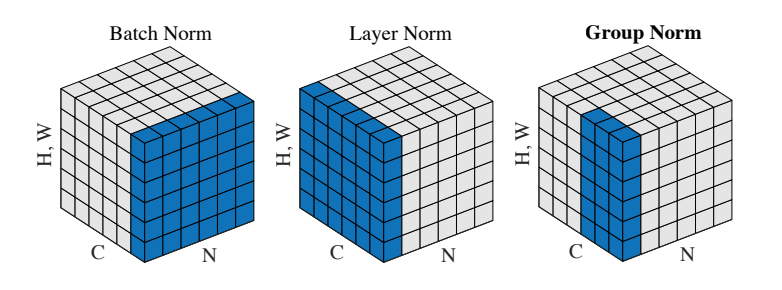
\includegraphics{normalization.png}

\textbf{Visual comparison of the normalization techniques discussed so
far (image edited from {[}5{]})}

Even though an assumption of equal contribution is still being made
within each group, the authors hypothesize that this is not as
problematic, as innate grouping arises within features for visual
recognition. One example they use to illustrate this is that many
high-performance handcrafted features in traditional Computer Vision
have terms that are explicitly grouped together. Take for example
Histogram of Oriented Gradients {[}6{]}-\/- after computing histograms
per spatially local block, each per-block histogram is normalized before
being concatenated together to form the final feature vector.

You will now implement Group Normalization. Note that this normalization
technique that you are to implement in the following cells was
introduced and published to arXiv \emph{less than a month ago} -\/- this
truly is still an ongoing and excitingly active field of research!

{[}4{]} {[}Ba, Jimmy Lei, Jamie Ryan Kiros, and Geoffrey E. Hinton.
"Layer Normalization." stat 1050 (2016):
21.{]}(https://arxiv.org/pdf/1607.06450.pdf)

{[}5{]} {[}Wu, Yuxin, and Kaiming He. "Group Normalization." arXiv
preprint arXiv:1803.08494 (2018).{]}(https://arxiv.org/abs/1803.08494)

{[}6{]} {[}N. Dalal and B. Triggs. Histograms of oriented gradients for
human detection. In Computer Vision and Pattern Recognition (CVPR),
2005.{]}(https://ieeexplore.ieee.org/abstract/document/1467360/)

    \subsection{Group normalization:
forward}\label{group-normalization-forward}

In the file \texttt{cs231n/layers.py}, implement the forward pass for
group normalization in the function
\texttt{spatial\_groupnorm\_forward}. Check your implementation by
running the following:

    \begin{Verbatim}[commandchars=\\\{\}]
{\color{incolor}In [{\color{incolor}23}]:} \PY{n}{np}\PY{o}{.}\PY{n}{random}\PY{o}{.}\PY{n}{seed}\PY{p}{(}\PY{l+m+mi}{231}\PY{p}{)}
         \PY{c+c1}{\PYZsh{} Check the training\PYZhy{}time forward pass by checking means and variances}
         \PY{c+c1}{\PYZsh{} of features both before and after spatial batch normalization}
         
         \PY{n}{N}\PY{p}{,} \PY{n}{C}\PY{p}{,} \PY{n}{H}\PY{p}{,} \PY{n}{W} \PY{o}{=} \PY{l+m+mi}{2}\PY{p}{,} \PY{l+m+mi}{6}\PY{p}{,} \PY{l+m+mi}{4}\PY{p}{,} \PY{l+m+mi}{5}
         \PY{n}{G} \PY{o}{=} \PY{l+m+mi}{2}
         \PY{n}{x} \PY{o}{=} \PY{l+m+mi}{4} \PY{o}{*} \PY{n}{np}\PY{o}{.}\PY{n}{random}\PY{o}{.}\PY{n}{randn}\PY{p}{(}\PY{n}{N}\PY{p}{,} \PY{n}{C}\PY{p}{,} \PY{n}{H}\PY{p}{,} \PY{n}{W}\PY{p}{)} \PY{o}{+} \PY{l+m+mi}{10}
         \PY{n}{x\PYZus{}g} \PY{o}{=} \PY{n}{x}\PY{o}{.}\PY{n}{reshape}\PY{p}{(}\PY{p}{(}\PY{n}{N}\PY{o}{*}\PY{n}{G}\PY{p}{,}\PY{o}{\PYZhy{}}\PY{l+m+mi}{1}\PY{p}{)}\PY{p}{)}
         \PY{n+nb}{print}\PY{p}{(}\PY{l+s+s1}{\PYZsq{}}\PY{l+s+s1}{Before spatial group normalization:}\PY{l+s+s1}{\PYZsq{}}\PY{p}{)}
         \PY{n+nb}{print}\PY{p}{(}\PY{l+s+s1}{\PYZsq{}}\PY{l+s+s1}{  Shape: }\PY{l+s+s1}{\PYZsq{}}\PY{p}{,} \PY{n}{x}\PY{o}{.}\PY{n}{shape}\PY{p}{)}
         \PY{n+nb}{print}\PY{p}{(}\PY{l+s+s1}{\PYZsq{}}\PY{l+s+s1}{  Means: }\PY{l+s+s1}{\PYZsq{}}\PY{p}{,} \PY{n}{x\PYZus{}g}\PY{o}{.}\PY{n}{mean}\PY{p}{(}\PY{n}{axis}\PY{o}{=}\PY{l+m+mi}{1}\PY{p}{)}\PY{p}{)}
         \PY{n+nb}{print}\PY{p}{(}\PY{l+s+s1}{\PYZsq{}}\PY{l+s+s1}{  Stds: }\PY{l+s+s1}{\PYZsq{}}\PY{p}{,} \PY{n}{x\PYZus{}g}\PY{o}{.}\PY{n}{std}\PY{p}{(}\PY{n}{axis}\PY{o}{=}\PY{l+m+mi}{1}\PY{p}{)}\PY{p}{)}
         
         \PY{c+c1}{\PYZsh{} Means should be close to zero and stds close to one}
         \PY{n}{gamma}\PY{p}{,} \PY{n}{beta} \PY{o}{=} \PY{n}{np}\PY{o}{.}\PY{n}{ones}\PY{p}{(}\PY{p}{(}\PY{l+m+mi}{1}\PY{p}{,}\PY{n}{C}\PY{p}{,}\PY{l+m+mi}{1}\PY{p}{,}\PY{l+m+mi}{1}\PY{p}{)}\PY{p}{)}\PY{p}{,} \PY{n}{np}\PY{o}{.}\PY{n}{zeros}\PY{p}{(}\PY{p}{(}\PY{l+m+mi}{1}\PY{p}{,}\PY{n}{C}\PY{p}{,}\PY{l+m+mi}{1}\PY{p}{,}\PY{l+m+mi}{1}\PY{p}{)}\PY{p}{)}
         \PY{n}{bn\PYZus{}param} \PY{o}{=} \PY{p}{\PYZob{}}\PY{l+s+s1}{\PYZsq{}}\PY{l+s+s1}{mode}\PY{l+s+s1}{\PYZsq{}}\PY{p}{:} \PY{l+s+s1}{\PYZsq{}}\PY{l+s+s1}{train}\PY{l+s+s1}{\PYZsq{}}\PY{p}{\PYZcb{}}
         
         \PY{n}{out}\PY{p}{,} \PY{n}{\PYZus{}} \PY{o}{=} \PY{n}{spatial\PYZus{}groupnorm\PYZus{}forward}\PY{p}{(}\PY{n}{x}\PY{p}{,} \PY{n}{gamma}\PY{p}{,} \PY{n}{beta}\PY{p}{,} \PY{n}{G}\PY{p}{,} \PY{n}{bn\PYZus{}param}\PY{p}{)}
         \PY{n}{out\PYZus{}g} \PY{o}{=} \PY{n}{out}\PY{o}{.}\PY{n}{reshape}\PY{p}{(}\PY{p}{(}\PY{n}{N}\PY{o}{*}\PY{n}{G}\PY{p}{,}\PY{o}{\PYZhy{}}\PY{l+m+mi}{1}\PY{p}{)}\PY{p}{)}
         \PY{n+nb}{print}\PY{p}{(}\PY{l+s+s1}{\PYZsq{}}\PY{l+s+s1}{After spatial group normalization:}\PY{l+s+s1}{\PYZsq{}}\PY{p}{)}
         \PY{n+nb}{print}\PY{p}{(}\PY{l+s+s1}{\PYZsq{}}\PY{l+s+s1}{  Shape: }\PY{l+s+s1}{\PYZsq{}}\PY{p}{,} \PY{n}{out}\PY{o}{.}\PY{n}{shape}\PY{p}{)}
         \PY{n+nb}{print}\PY{p}{(}\PY{l+s+s1}{\PYZsq{}}\PY{l+s+s1}{  Means: }\PY{l+s+s1}{\PYZsq{}}\PY{p}{,} \PY{n}{out\PYZus{}g}\PY{o}{.}\PY{n}{mean}\PY{p}{(}\PY{n}{axis}\PY{o}{=}\PY{l+m+mi}{1}\PY{p}{)}\PY{p}{)}
         \PY{n+nb}{print}\PY{p}{(}\PY{l+s+s1}{\PYZsq{}}\PY{l+s+s1}{  Stds: }\PY{l+s+s1}{\PYZsq{}}\PY{p}{,} \PY{n}{out\PYZus{}g}\PY{o}{.}\PY{n}{std}\PY{p}{(}\PY{n}{axis}\PY{o}{=}\PY{l+m+mi}{1}\PY{p}{)}\PY{p}{)}
\end{Verbatim}


    \begin{Verbatim}[commandchars=\\\{\}]
Before spatial group normalization:
  Shape:  (2, 6, 4, 5)
  Means:  [9.72505327 8.51114185 8.9147544  9.43448077]
  Stds:  [3.67070958 3.09892597 4.27043622 3.97521327]
After spatial group normalization:
  Shape:  (2, 6, 4, 5)
  Means:  [ 0.13335201 -0.0708835  -0.13335201  0.0708835 ]
  Stds:  [0.99083728 0.99376409 0.99083728 0.99376409]

    \end{Verbatim}

    \subsection{Spatial group normalization:
backward}\label{spatial-group-normalization-backward}

In the file \texttt{cs231n/layers.py}, implement the backward pass for
spatial batch normalization in the function
\texttt{spatial\_groupnorm\_backward}. Run the following to check your
implementation using a numeric gradient check:

    \begin{Verbatim}[commandchars=\\\{\}]
{\color{incolor}In [{\color{incolor}24}]:} \PY{n}{np}\PY{o}{.}\PY{n}{random}\PY{o}{.}\PY{n}{seed}\PY{p}{(}\PY{l+m+mi}{231}\PY{p}{)}
         \PY{n}{N}\PY{p}{,} \PY{n}{C}\PY{p}{,} \PY{n}{H}\PY{p}{,} \PY{n}{W} \PY{o}{=} \PY{l+m+mi}{2}\PY{p}{,} \PY{l+m+mi}{6}\PY{p}{,} \PY{l+m+mi}{4}\PY{p}{,} \PY{l+m+mi}{5}
         \PY{n}{G} \PY{o}{=} \PY{l+m+mi}{2}
         \PY{n}{x} \PY{o}{=} \PY{l+m+mi}{5} \PY{o}{*} \PY{n}{np}\PY{o}{.}\PY{n}{random}\PY{o}{.}\PY{n}{randn}\PY{p}{(}\PY{n}{N}\PY{p}{,} \PY{n}{C}\PY{p}{,} \PY{n}{H}\PY{p}{,} \PY{n}{W}\PY{p}{)} \PY{o}{+} \PY{l+m+mi}{12}
         \PY{n}{gamma} \PY{o}{=} \PY{n}{np}\PY{o}{.}\PY{n}{random}\PY{o}{.}\PY{n}{randn}\PY{p}{(}\PY{l+m+mi}{1}\PY{p}{,}\PY{n}{C}\PY{p}{,}\PY{l+m+mi}{1}\PY{p}{,}\PY{l+m+mi}{1}\PY{p}{)}
         \PY{n}{beta} \PY{o}{=} \PY{n}{np}\PY{o}{.}\PY{n}{random}\PY{o}{.}\PY{n}{randn}\PY{p}{(}\PY{l+m+mi}{1}\PY{p}{,}\PY{n}{C}\PY{p}{,}\PY{l+m+mi}{1}\PY{p}{,}\PY{l+m+mi}{1}\PY{p}{)}
         \PY{n}{dout} \PY{o}{=} \PY{n}{np}\PY{o}{.}\PY{n}{random}\PY{o}{.}\PY{n}{randn}\PY{p}{(}\PY{n}{N}\PY{p}{,} \PY{n}{C}\PY{p}{,} \PY{n}{H}\PY{p}{,} \PY{n}{W}\PY{p}{)}
         
         \PY{n}{gn\PYZus{}param} \PY{o}{=} \PY{p}{\PYZob{}}\PY{p}{\PYZcb{}}
         \PY{n}{fx} \PY{o}{=} \PY{k}{lambda} \PY{n}{x}\PY{p}{:} \PY{n}{spatial\PYZus{}groupnorm\PYZus{}forward}\PY{p}{(}\PY{n}{x}\PY{p}{,} \PY{n}{gamma}\PY{p}{,} \PY{n}{beta}\PY{p}{,} \PY{n}{G}\PY{p}{,} \PY{n}{gn\PYZus{}param}\PY{p}{)}\PY{p}{[}\PY{l+m+mi}{0}\PY{p}{]}
         \PY{n}{fg} \PY{o}{=} \PY{k}{lambda} \PY{n}{a}\PY{p}{:} \PY{n}{spatial\PYZus{}groupnorm\PYZus{}forward}\PY{p}{(}\PY{n}{x}\PY{p}{,} \PY{n}{gamma}\PY{p}{,} \PY{n}{beta}\PY{p}{,} \PY{n}{G}\PY{p}{,} \PY{n}{gn\PYZus{}param}\PY{p}{)}\PY{p}{[}\PY{l+m+mi}{0}\PY{p}{]}
         \PY{n}{fb} \PY{o}{=} \PY{k}{lambda} \PY{n}{b}\PY{p}{:} \PY{n}{spatial\PYZus{}groupnorm\PYZus{}forward}\PY{p}{(}\PY{n}{x}\PY{p}{,} \PY{n}{gamma}\PY{p}{,} \PY{n}{beta}\PY{p}{,} \PY{n}{G}\PY{p}{,} \PY{n}{gn\PYZus{}param}\PY{p}{)}\PY{p}{[}\PY{l+m+mi}{0}\PY{p}{]}
         
         \PY{n}{dx\PYZus{}num} \PY{o}{=} \PY{n}{eval\PYZus{}numerical\PYZus{}gradient\PYZus{}array}\PY{p}{(}\PY{n}{fx}\PY{p}{,} \PY{n}{x}\PY{p}{,} \PY{n}{dout}\PY{p}{)}
         \PY{n}{da\PYZus{}num} \PY{o}{=} \PY{n}{eval\PYZus{}numerical\PYZus{}gradient\PYZus{}array}\PY{p}{(}\PY{n}{fg}\PY{p}{,} \PY{n}{gamma}\PY{p}{,} \PY{n}{dout}\PY{p}{)}
         \PY{n}{db\PYZus{}num} \PY{o}{=} \PY{n}{eval\PYZus{}numerical\PYZus{}gradient\PYZus{}array}\PY{p}{(}\PY{n}{fb}\PY{p}{,} \PY{n}{beta}\PY{p}{,} \PY{n}{dout}\PY{p}{)}
         
         \PY{n}{\PYZus{}}\PY{p}{,} \PY{n}{cache} \PY{o}{=} \PY{n}{spatial\PYZus{}groupnorm\PYZus{}forward}\PY{p}{(}\PY{n}{x}\PY{p}{,} \PY{n}{gamma}\PY{p}{,} \PY{n}{beta}\PY{p}{,} \PY{n}{G}\PY{p}{,} \PY{n}{gn\PYZus{}param}\PY{p}{)}
         \PY{n}{dx}\PY{p}{,} \PY{n}{dgamma}\PY{p}{,} \PY{n}{dbeta} \PY{o}{=} \PY{n}{spatial\PYZus{}groupnorm\PYZus{}backward}\PY{p}{(}\PY{n}{dout}\PY{p}{,} \PY{n}{cache}\PY{p}{)}
         \PY{c+c1}{\PYZsh{}You should expect errors of magnitudes between 1e\PYZhy{}12\PYZti{}1e\PYZhy{}07}
         \PY{n+nb}{print}\PY{p}{(}\PY{l+s+s1}{\PYZsq{}}\PY{l+s+s1}{dx error: }\PY{l+s+s1}{\PYZsq{}}\PY{p}{,} \PY{n}{rel\PYZus{}error}\PY{p}{(}\PY{n}{dx\PYZus{}num}\PY{p}{,} \PY{n}{dx}\PY{p}{)}\PY{p}{)}
         \PY{n+nb}{print}\PY{p}{(}\PY{l+s+s1}{\PYZsq{}}\PY{l+s+s1}{dgamma error: }\PY{l+s+s1}{\PYZsq{}}\PY{p}{,} \PY{n}{rel\PYZus{}error}\PY{p}{(}\PY{n}{da\PYZus{}num}\PY{p}{,} \PY{n}{dgamma}\PY{p}{)}\PY{p}{)}
         \PY{n+nb}{print}\PY{p}{(}\PY{l+s+s1}{\PYZsq{}}\PY{l+s+s1}{dbeta error: }\PY{l+s+s1}{\PYZsq{}}\PY{p}{,} \PY{n}{rel\PYZus{}error}\PY{p}{(}\PY{n}{db\PYZus{}num}\PY{p}{,} \PY{n}{dbeta}\PY{p}{)}\PY{p}{)}
\end{Verbatim}


    \begin{Verbatim}[commandchars=\\\{\}]
dx error:  0.0010103963079019869
dgamma error:  1.0
dbeta error:  1.0

    \end{Verbatim}


    % Add a bibliography block to the postdoc
    
    
    
    \end{document}
